\documentclass{beamer}
\usetheme{Malmoe}
%\usepackage{beamerthemesplit} %// Activate for custom appearance
%\setbeamertemplate{footline}[page number]{}
\usepackage{graphicx,subfig,float}


\title{Kobe Bryant Shot Selection}
%\author{K.I. Chung, K.J. Yang}
\author[K.I. Chung, K.J. Yang]{K.I. Chung, K.J. Yang\\{\small Supervised by: Prof. Guo, Mei-Hui }}
\date{January 14, 2017}

\begin{document}

\frame{\titlepage}
%%%% outline %%%%
\section[Outline]{}
\frame{\tableofcontents}
 
% %%%  introduction %%%%
\section{Introduction}
%% Overview of the Data %%
\subsection{Overview of the Data}

\frame
{
  	\frametitle{About the data}
	\begin{columns}
		\begin{column}{0.5\textwidth}
			\begin{itemize}
				\item {From the Kaggle}
				\item{Containing all the Kobe's shots during his career}
				\item{30697 shots and 25 variables}
				\item{25697 training data and 5000 test data}
			\end{itemize}

		\end{column}
  		\begin{column}{0.5\textwidth}
			\begin{figure}
    				\begin{center}
        					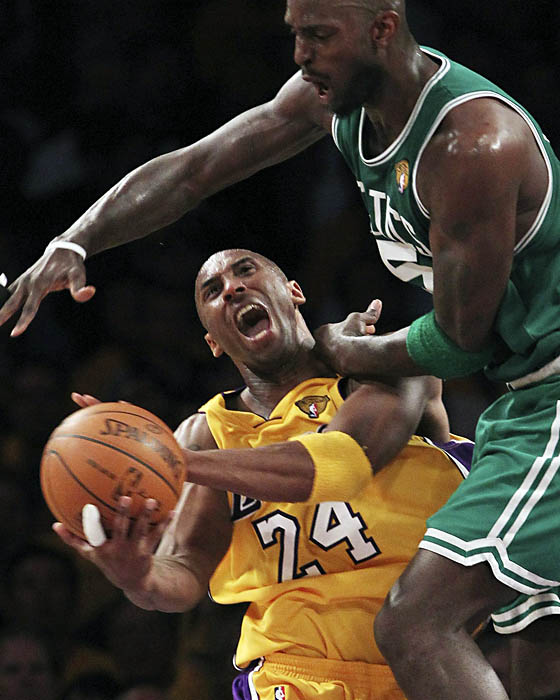
\includegraphics[width=130pt]{figure/Kobe_1.png}
        					\caption{Kobe Bryant was blocked}
       					\label{}
    				\end{center}
			\end{figure}
		\end{column}
	\end{columns}
}

\frame
{
  	\frametitle{Response}
	\begin{columns}
		\begin{column}{0.5\textwidth}
			\begin{itemize}
				\item {Whether a shot is made or not}
				\item{1 and 0 are denoted for a shot is made or not}
				\item{NA is denoted for the test data}
			\end{itemize}

		\end{column}
  		\begin{column}{0.5\textwidth}
			\begin{figure}
    				\begin{center}
        					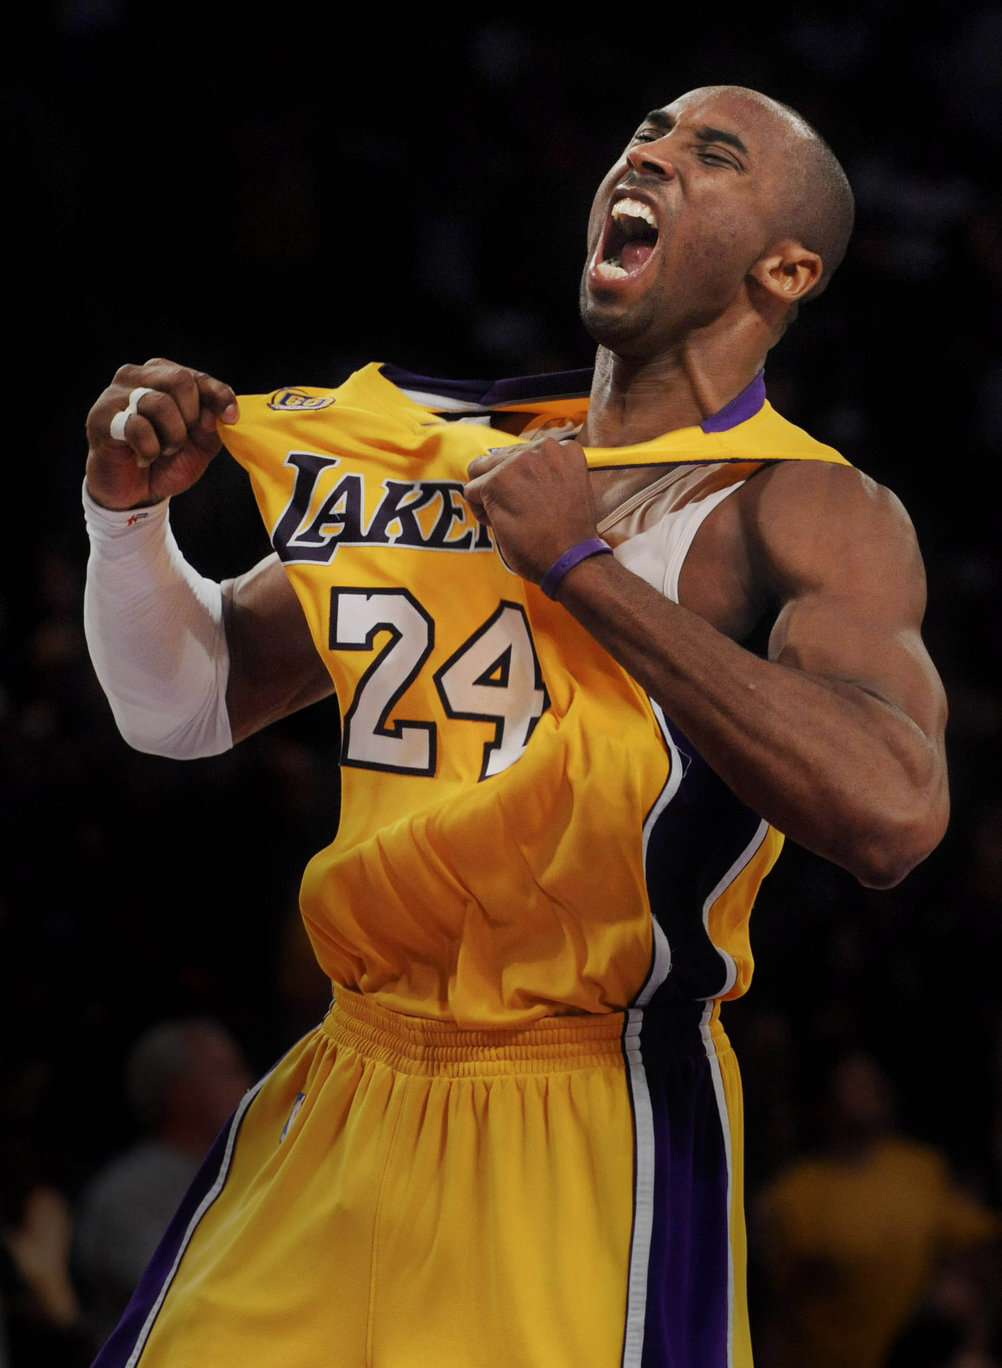
\includegraphics[width=110pt]{figure/Kobe_2.png}
        					\caption{Kobe Bryant was in a rage}
       					\label{}
    				\end{center}
			\end{figure}
		\end{column}
	\end{columns}
}

\frame
{
  	\frametitle{Predictors}
	\begin{columns}
		\begin{column}{0.5\textwidth}
			\begin{itemize}
				\item {24 variables}
				\item{Factors: shot types, shot zone, match up, playoffs?}
				\item{Continuous: location(x, y),  time remaining?}
			\end{itemize}

		\end{column}
  		\begin{column}{0.5\textwidth}
			\begin{figure}
    				\begin{center}
        					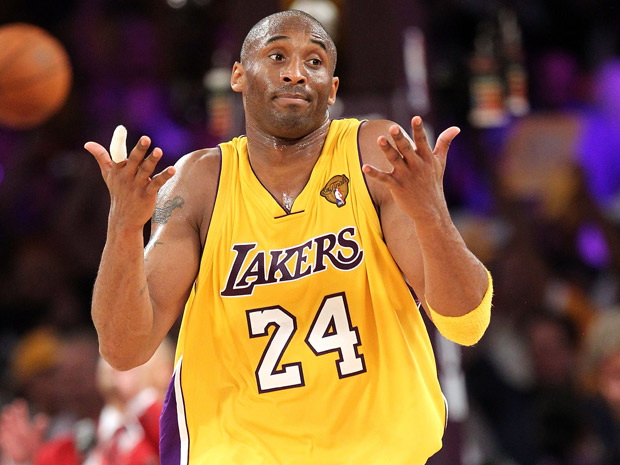
\includegraphics[width=160pt]{figure/Kobe_3.png}
        					\caption{Kobe Bryant did not care}
       					\label{}
    				\end{center}
			\end{figure}
		\end{column}
	\end{columns}
}

%% Summary of the Data %%
\frame{
	\begin{figure}
    		\begin{center}
        			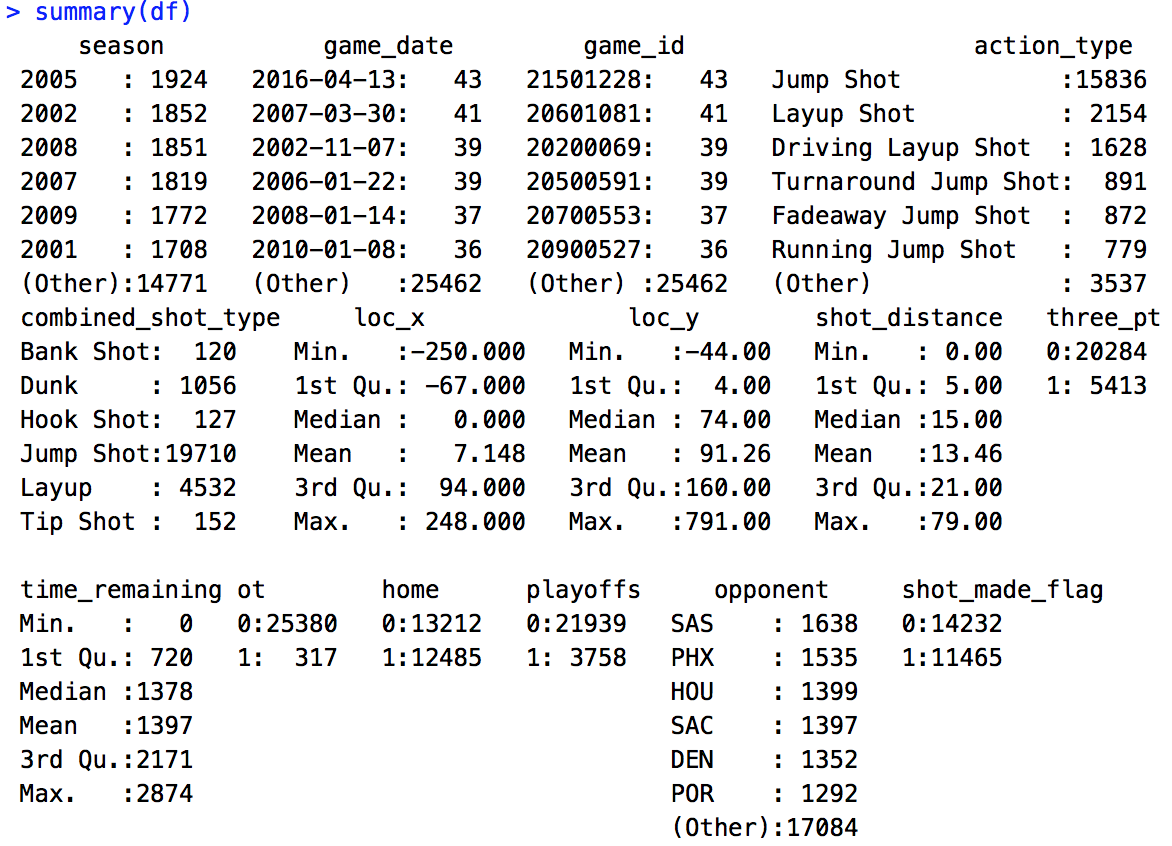
\includegraphics[width=270pt]{figure/f00_summary.png}
    		\end{center}
	\end{figure}
}

%% Comparisons and Hypothesis Tests %%
\subsection{Comparisons and Hypothesis Tests}
\frame{
	\frametitle{Home v.s. Away}
  	\begin{columns}
		\begin{column}{0.5\textwidth}
			\begin{itemize}
				\item{paired: FALSE}
				\item{p-value of variance test: 0.7318}
				\item{var.equal: TRUE}
				\item{p-value of two sample t-test:0.0007103}
				\item{result: different means}
			\end{itemize}

		\end{column}
  		\begin{column}{0.5\textwidth}
			\begin{figure}
    				\begin{center}
        					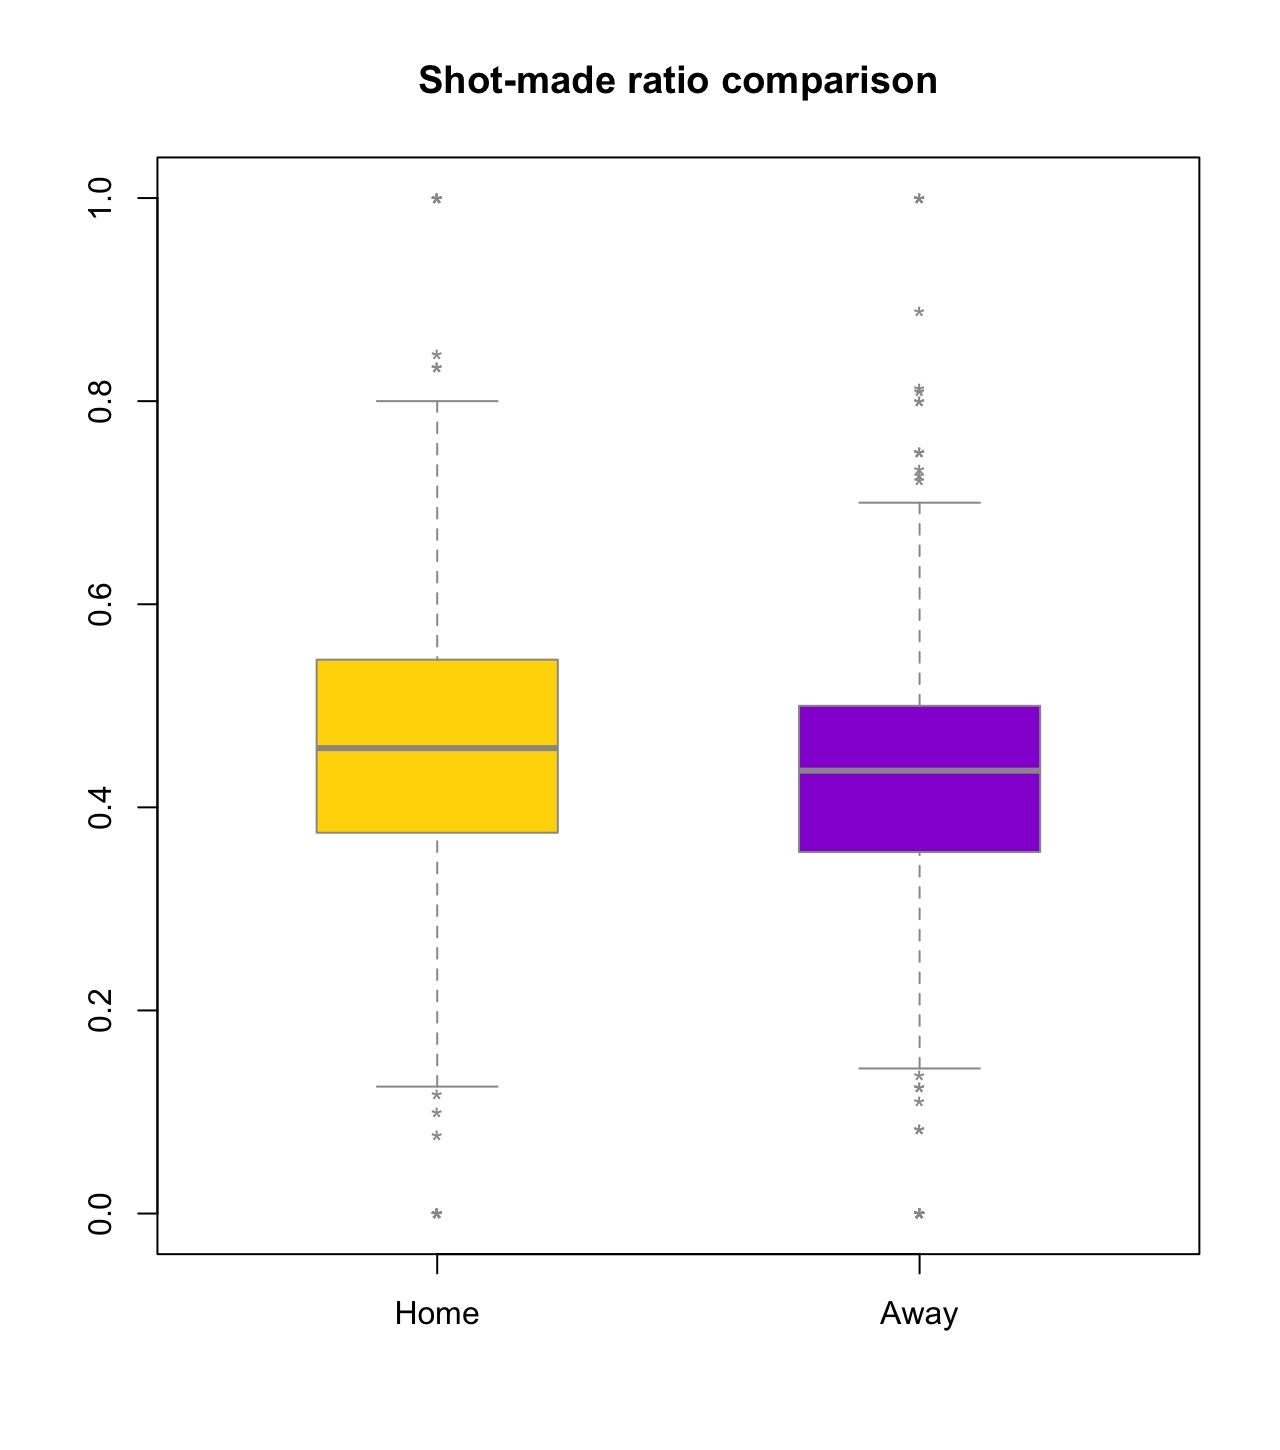
\includegraphics[width=140pt]{figure/f06_compare_home.png}
    				\end{center}
			\end{figure}
		\end{column}
	\end{columns}
}

\frame{
	\frametitle{Regular games v.s. Playoffs}
  	\begin{columns}
		\begin{column}{0.5\textwidth}
			\begin{itemize}
				\item{paired: FALSE}
				\item{p-value of variance test: 0.2206}
				\item{var.equal: TRUE}
				\item{p-value of two sample t-test:0.5658}
				\item{result: same means}
			\end{itemize}

		\end{column}
  		\begin{column}{0.5\textwidth}
			\begin{figure}
    				\begin{center}
        					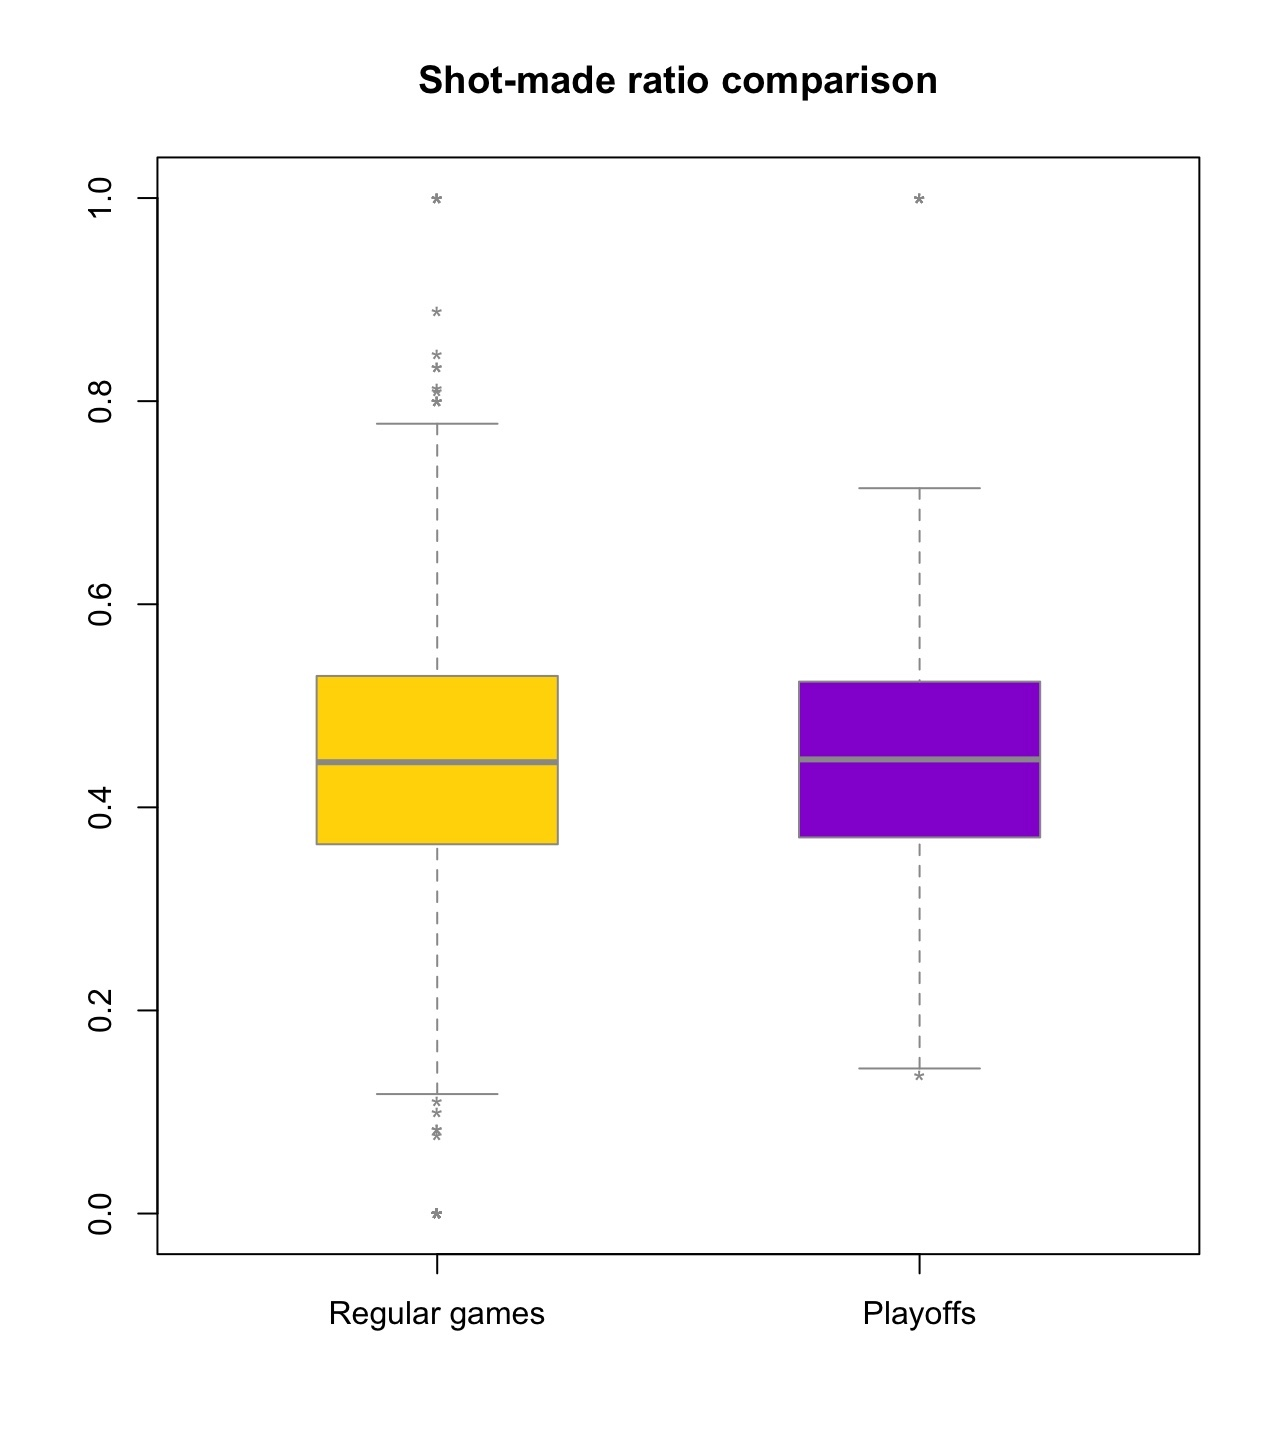
\includegraphics[width=140pt]{figure/f07_compare_playoffs.png}
    				\end{center}
			\end{figure}
		\end{column}
	\end{columns}
}

\frame{
	\frametitle{2-pt. v.s. 3-pt. }
  	\begin{columns}
		\begin{column}{0.5\textwidth}
			\begin{itemize}
				\item{paired: TRUE}
				\item{p-value of variance test: 0}
				\item{var.equal: FALSE}
				\item{p-value of two sample t-test: 0}
				\item{result: different means}
			\end{itemize}

		\end{column}
  		\begin{column}{0.5\textwidth}
			\begin{figure}
    				\begin{center}
        					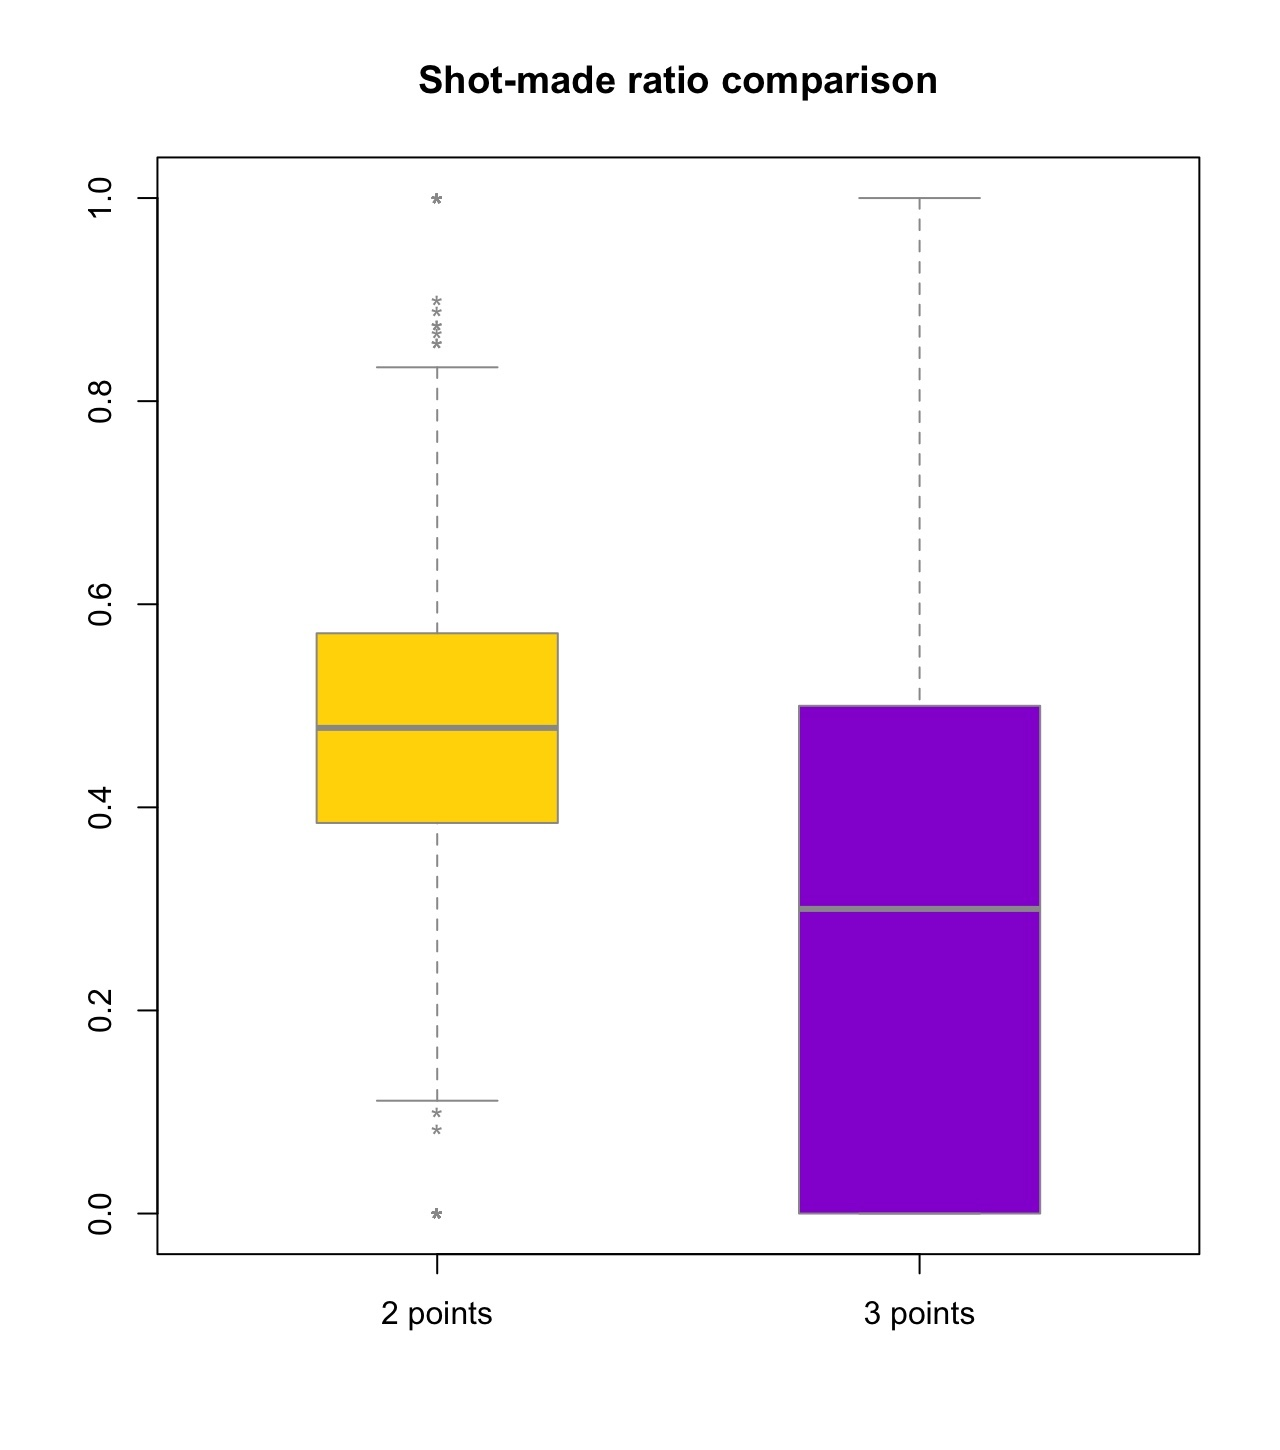
\includegraphics[width=140pt]{figure/f08_compare_three.png}
    				\end{center}
			\end{figure}
		\end{column}
	\end{columns}
}

\frame{
	\frametitle{Made Shot Location Comparison}
	\begin{figure}
    		\begin{center}
        			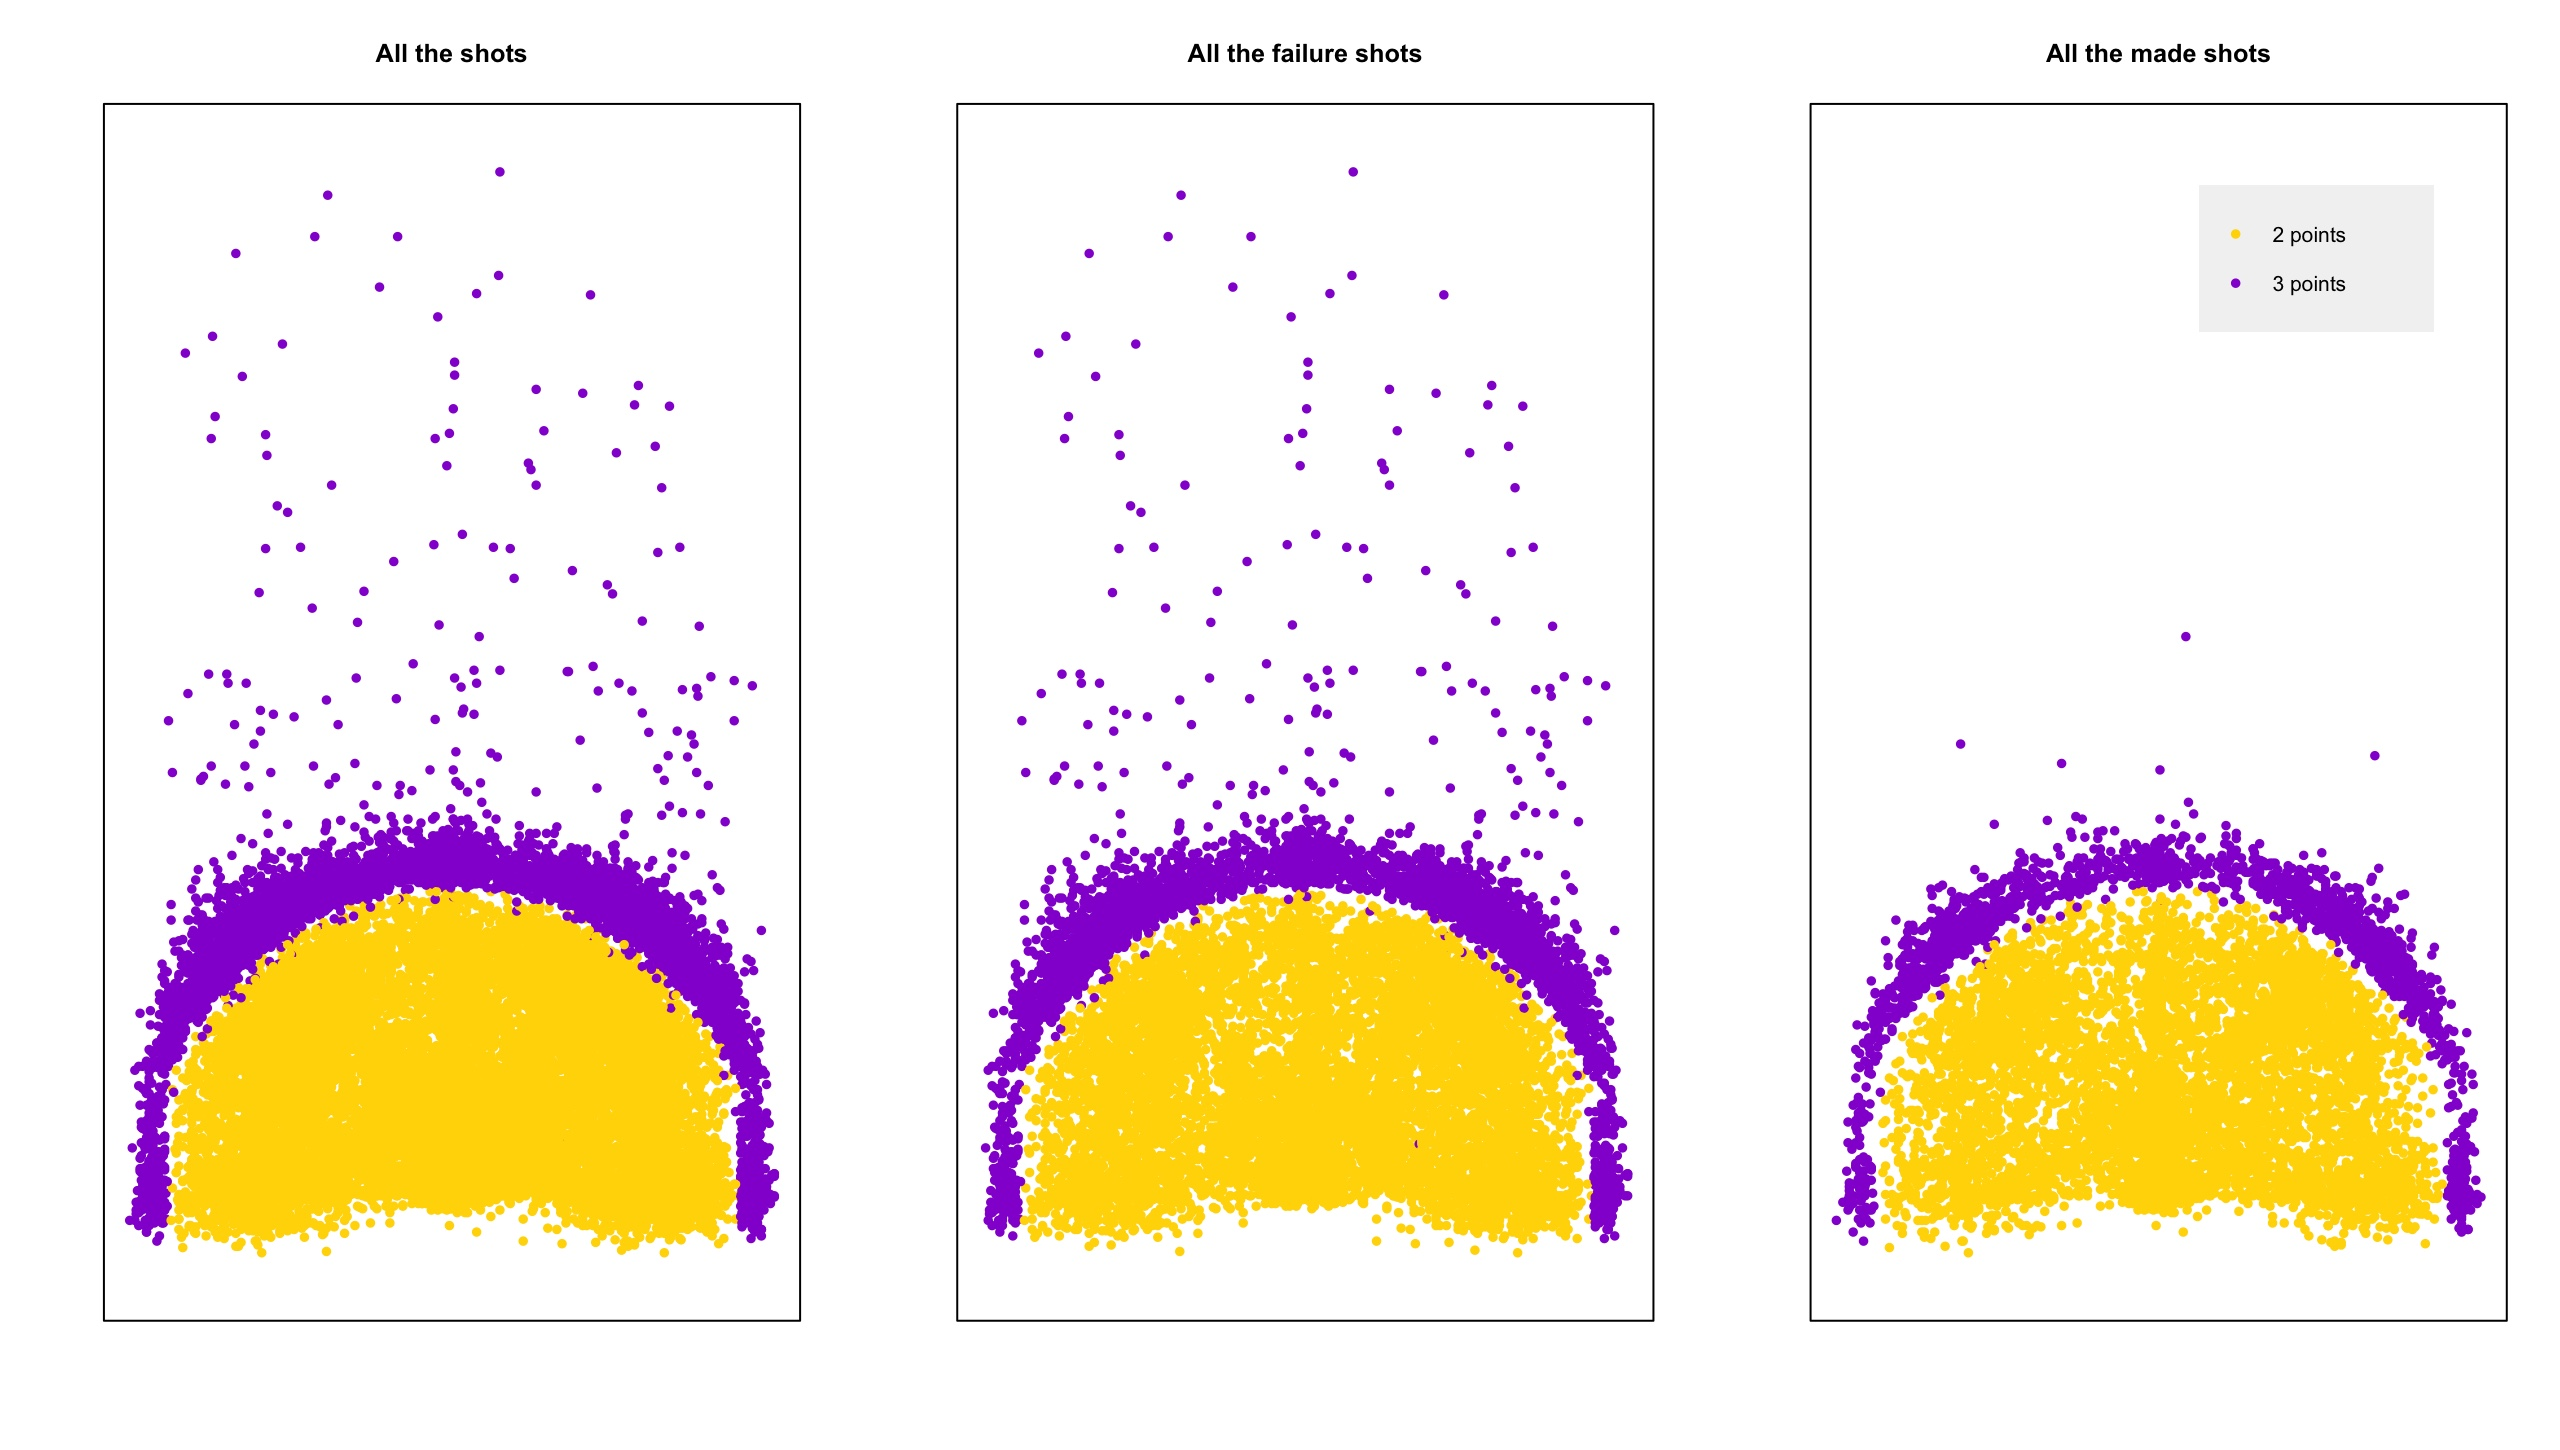
\includegraphics[width=300pt]{figure/f03_shot_loc.png}
    		\end{center}
	\end{figure}
}

\section{Statistical Analysis}
%%%% KNN %%%%
\subsection{KNN Classifier}
\frame{
\frametitle{Yearly Trend of the KNN Classifier}
	\begin{figure}
    		\begin{center}
        			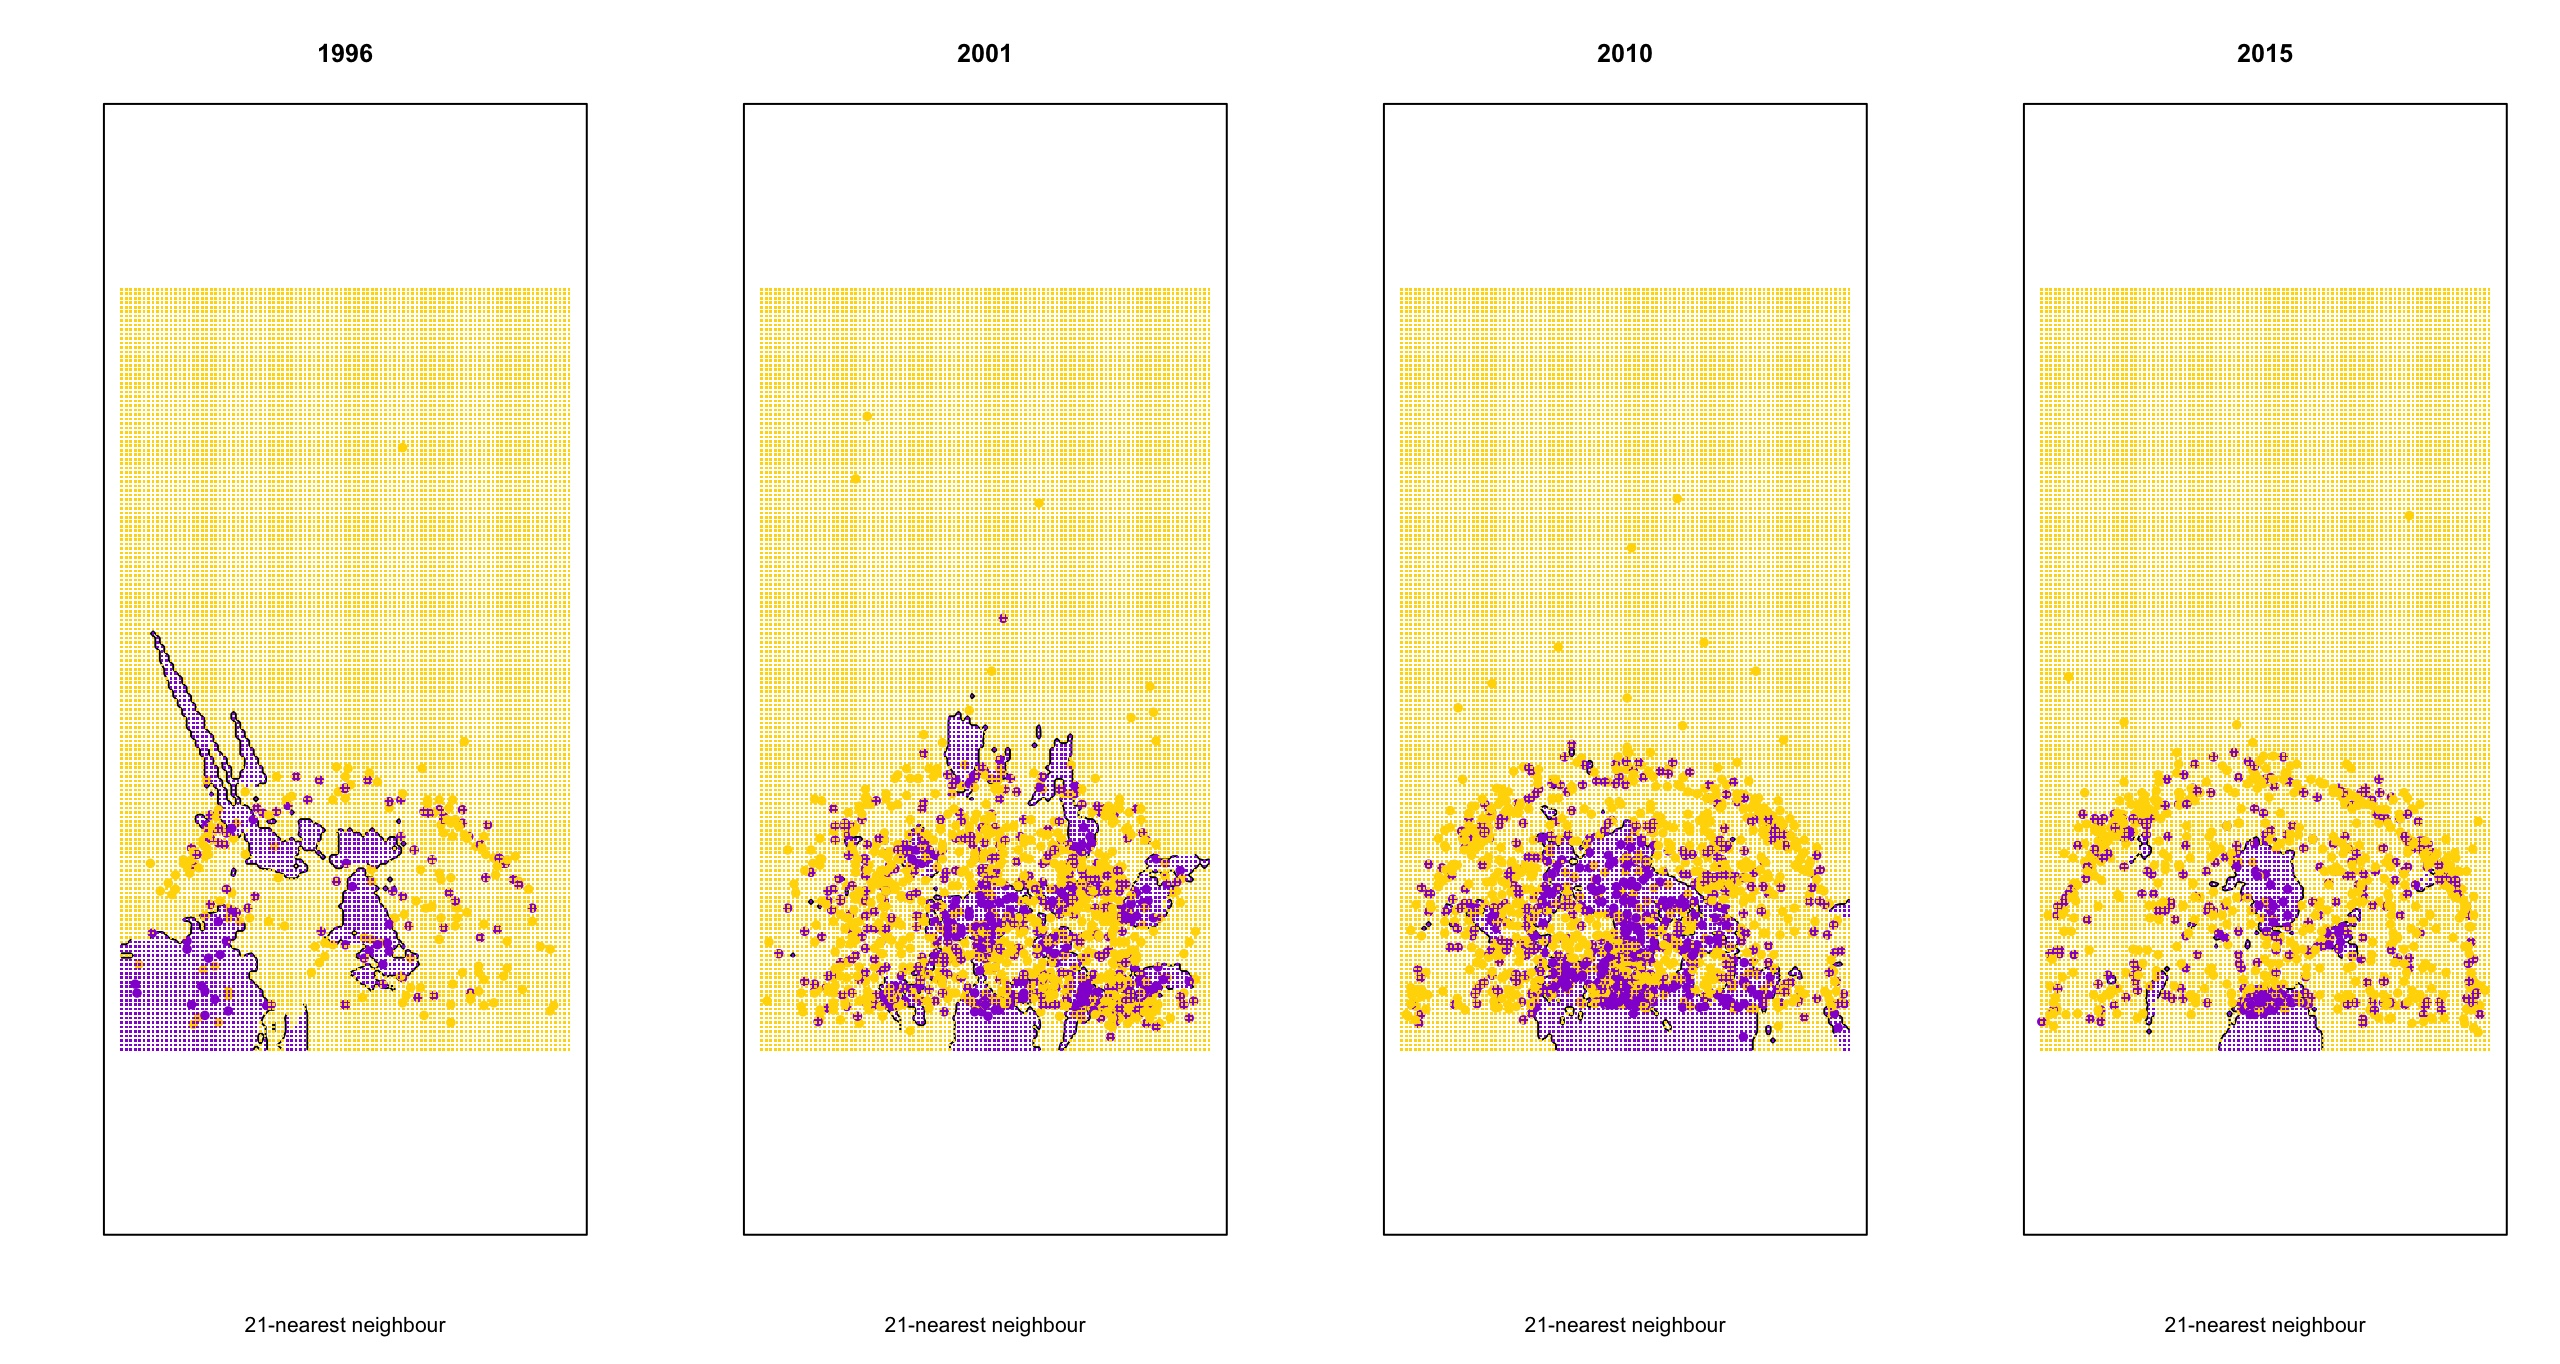
\includegraphics[width=300pt]{figure/f01_KNN_year.png}
    		\end{center}
	\end{figure}
}


\frame{
\frametitle{KNN Results with Different k}
	\begin{figure}
    		\begin{center}
        			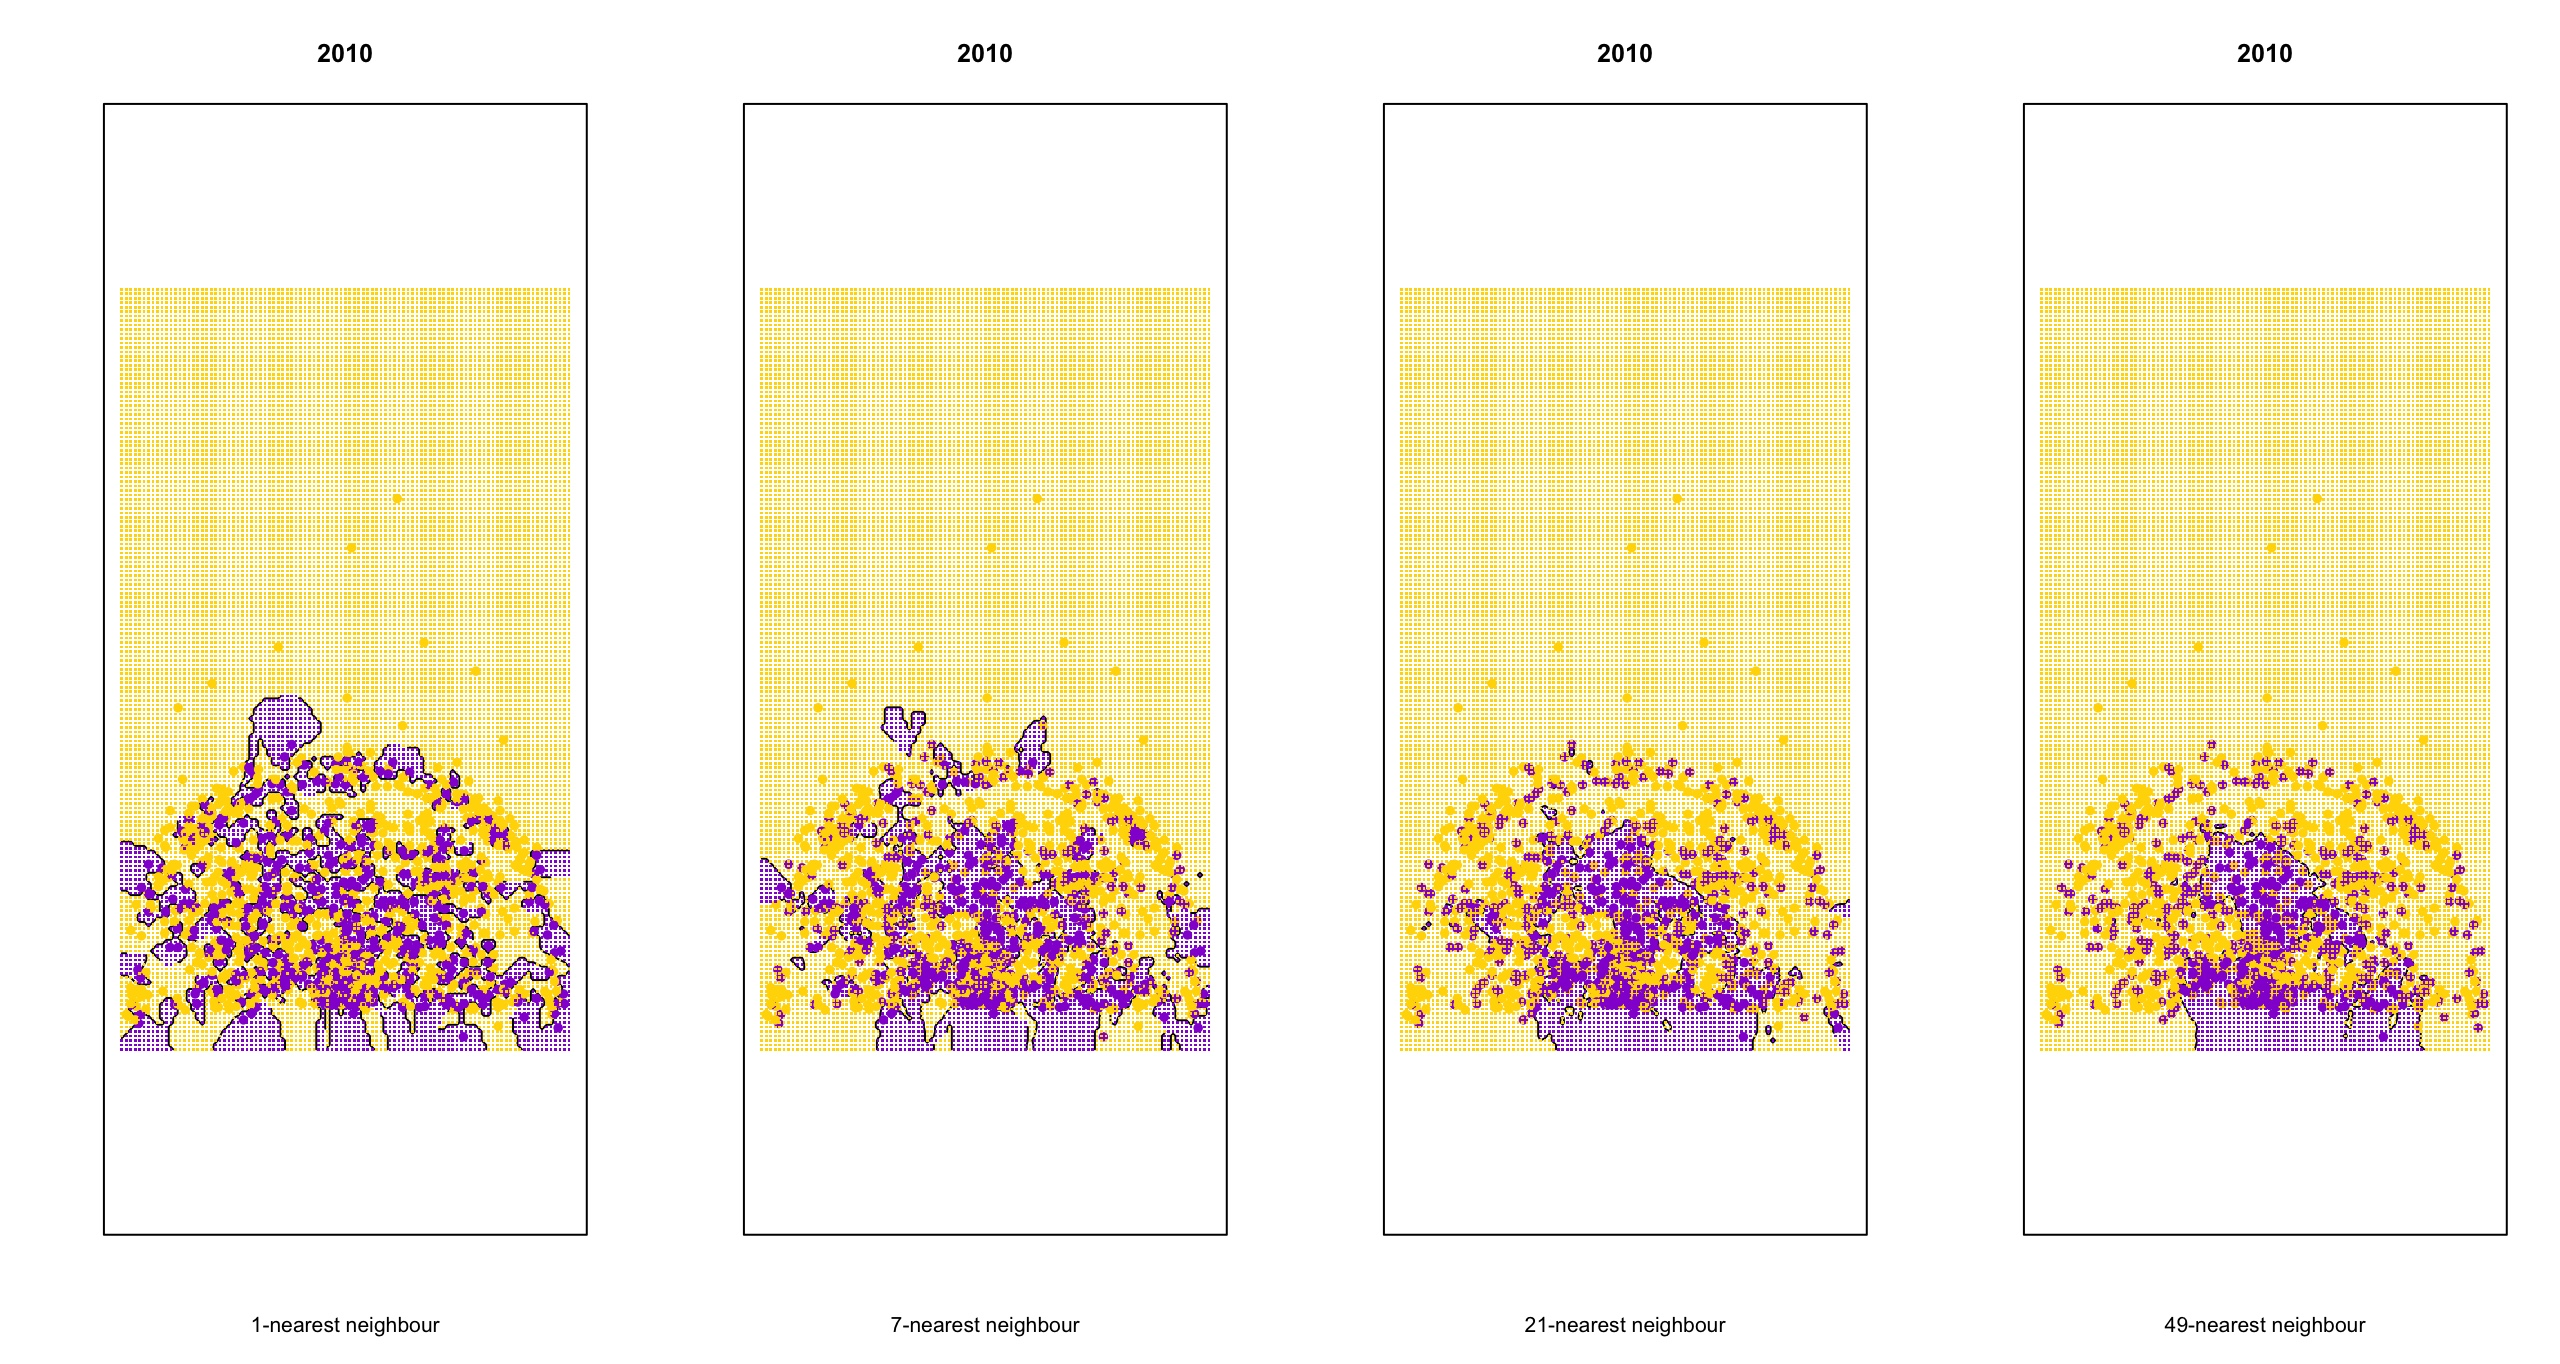
\includegraphics[width=300pt]{figure/f02_KNN_k.png}
    		\end{center}
	\end{figure}
}

\frame{
\frametitle{20-folds Cross Validation Result in Different Season}
	\begin{figure}
    		\begin{center}
        			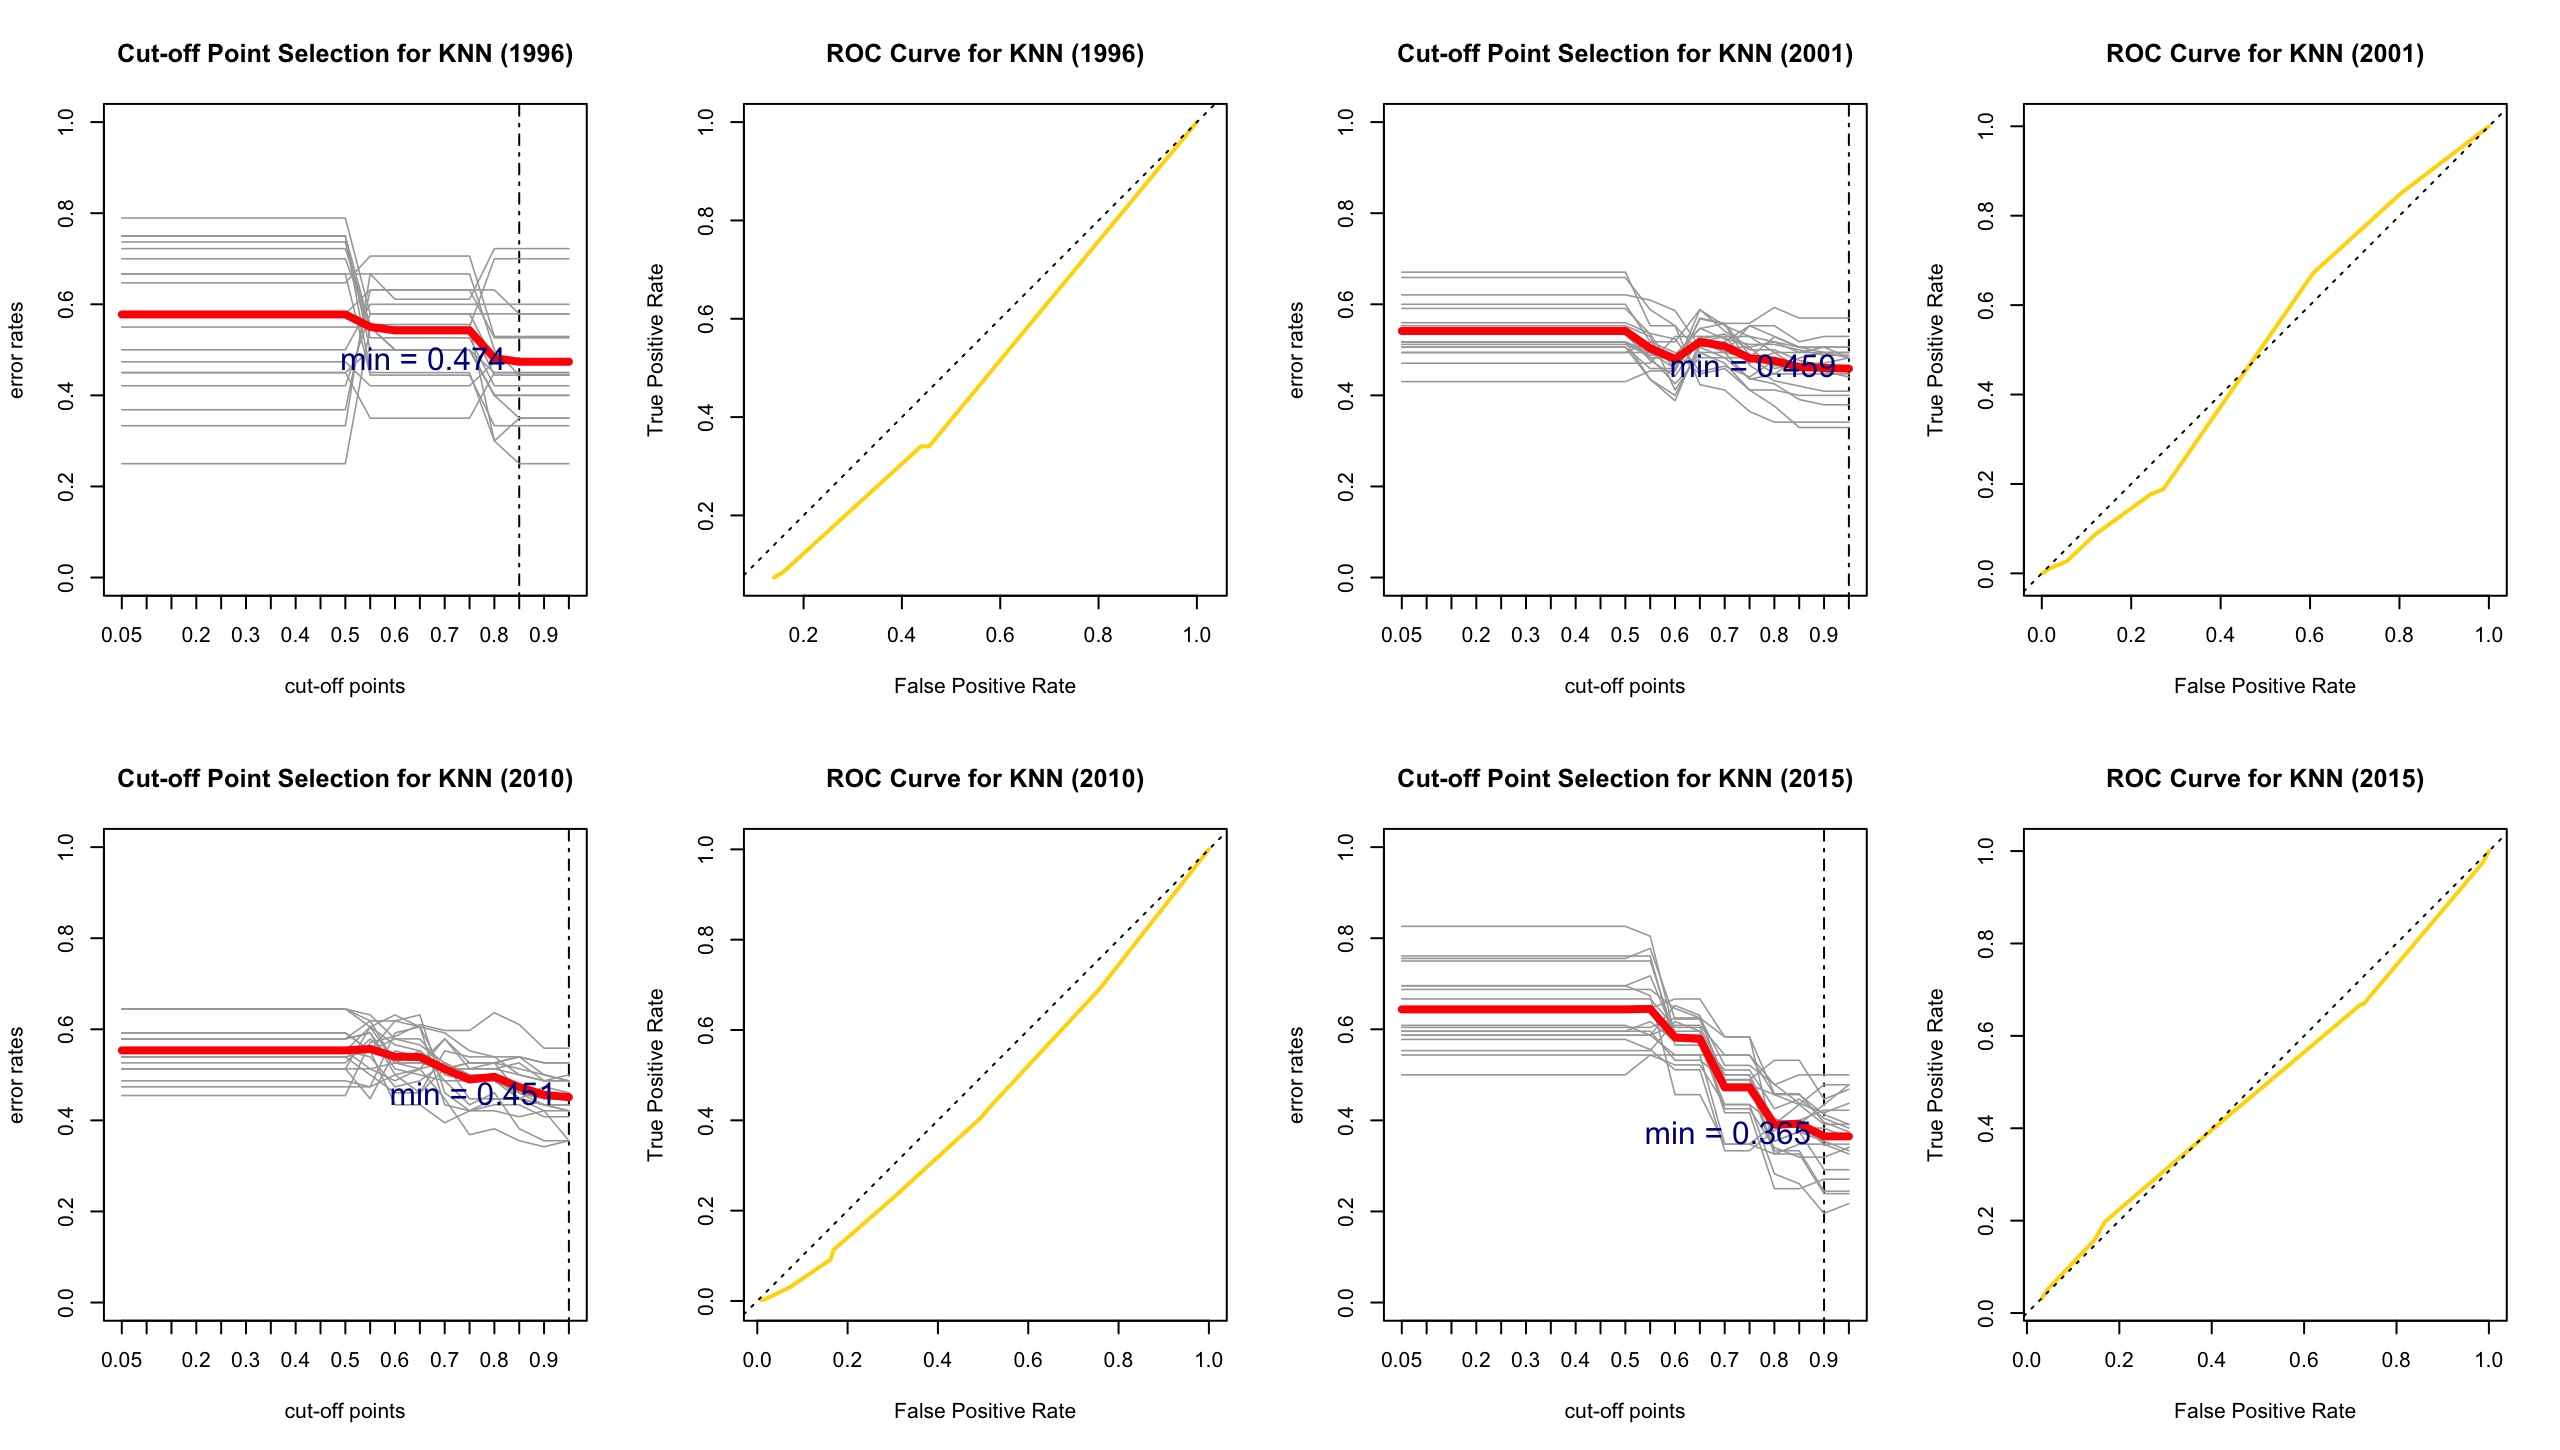
\includegraphics[width=300pt]{figure/f10_KNN_err.png}
    		\end{center}
	\end{figure}
}

%% Logistic Regression %%

%% mixed %%
\subsection{Mixed Model Selection for Logistic Regression}
% mixed 1 %
\frame{
\qquad With the mixed selection method , the following predictors were chosen.\\
	\begin{columns}
		\begin{column}{0.5\textwidth}
			\begin{itemize}
				\item{season}
				\item{combined\_shot\_ type}
				\item{loc\_y}
				\item{shot\_distance}
			\end{itemize}
		\end{column}		
		\begin{column}{0.5\textwidth}
			\begin{itemize}
				\item{three\_pt}
				\item{time\_remaining}
				\item{home}
			\end{itemize}	
		\end{column}	
	\end{columns}
}

% mixed 2 %
\frame{
\qquad Now we check the collinearity, the result is shown below. We can noticed that the predictors location y, shot distance and three point have relatively high collinearity. \\
\begin{equation*}
	GVIF' = GVIF^{\frac{1}{2df}}
\end{equation*}

\begin{table}[htp]
		\begin{center}
			\begin{tabular}{lrrr}
	                      	predictor			&	GVIF 		&	df 		&	GVIF'			\\
				\hline
				season             		&	1.0772		&	19     	&	1.0019			\\
				shot type 			&	2.9098 	  	&	5       	&	1.1127			\\
				location y			&	3.0372		&	1		&	\alert{1.7428}		\\	
				shot distance      	&	6.9311	  	&	1      		&	\alert{2.6327}		\\
				three point		&	2.2918		&	1		&	\alert{1.5139}		\\
				time remaining     	&	1.0176  		&	1        	&	1.0088			\\
				home               		&	1.0090	  	&	1        	&	1.0045			\\
			\end{tabular}
		\end{center}
	\label{default}
\end{table}
}

% mixed 3 %
\frame{
\qquad To eliminate the the effect of the collinearity, we will perform the "leave-one-in" model selection which provide us the least AIC model with one of three collinear predictors.
\begin{table}[htp]
	\caption{default}
		\begin{center}
			\begin{tabular}{lrrr}
	                      	predictor			&	location y 		&	shot distance 	&	three point	\\
				AIC               		&	33540.53	  	&	\alert{33466.69}       	&	33493.91		\\
			\end{tabular}
		\end{center}
	\label{default}
\end{table}

}

% mixed 4 %
\frame{
\begin{table}[htp]
	\caption{Coefficients of the Selected Predictors without Collinearity}
		\begin{center}
			\begin{tabular}{rrrrr}
	Intercept 	&	1997 		&	1998			&	1999		&	2000		\\ 
	1.2131    	&	-0.0367     	&	0.1537     		&	0.1611     	&	0.1874 	\\ \hline \hline
	2001 	&	2002			&	2003			&	2004		&	2005		\\ 
	0.1397     	&	0.1017     		&	0.0515     		&	0.1003     	&	0.2651 	\\ \hline \hline
	2006		&	2007			&	2008			&	2009		&	2010		\\
	0.2487     	&	0.2421     		&	0.2673     		&	0.2188     	&	0.2018      \\ \hline \hline
	2011		&	2012			&	2013			&	2014		&	2015		\\
	0.1482      &	0.244     		&	0.0589    		&	-0.0236     &	-0.042	\\ \hline \hline
	Dunk 	&	Shot			&	Jump Shot	&	Layup	&	Tip Shot	\\	
	1.0643  	&	-1.2381		&	-1.5344           	&	-1.2354	&	-2.1032 	\\ \hline \hline
	Distance	&	Time			&	Home		&			&			\\
	-0.0241	&	0.0004		&	0.0417		&			&			\\
			\end{tabular}
		\end{center}
	\label{default}
\end{table}
}

% mixed 5 %
\frame{
	\begin{figure}
    		\begin{center}
        			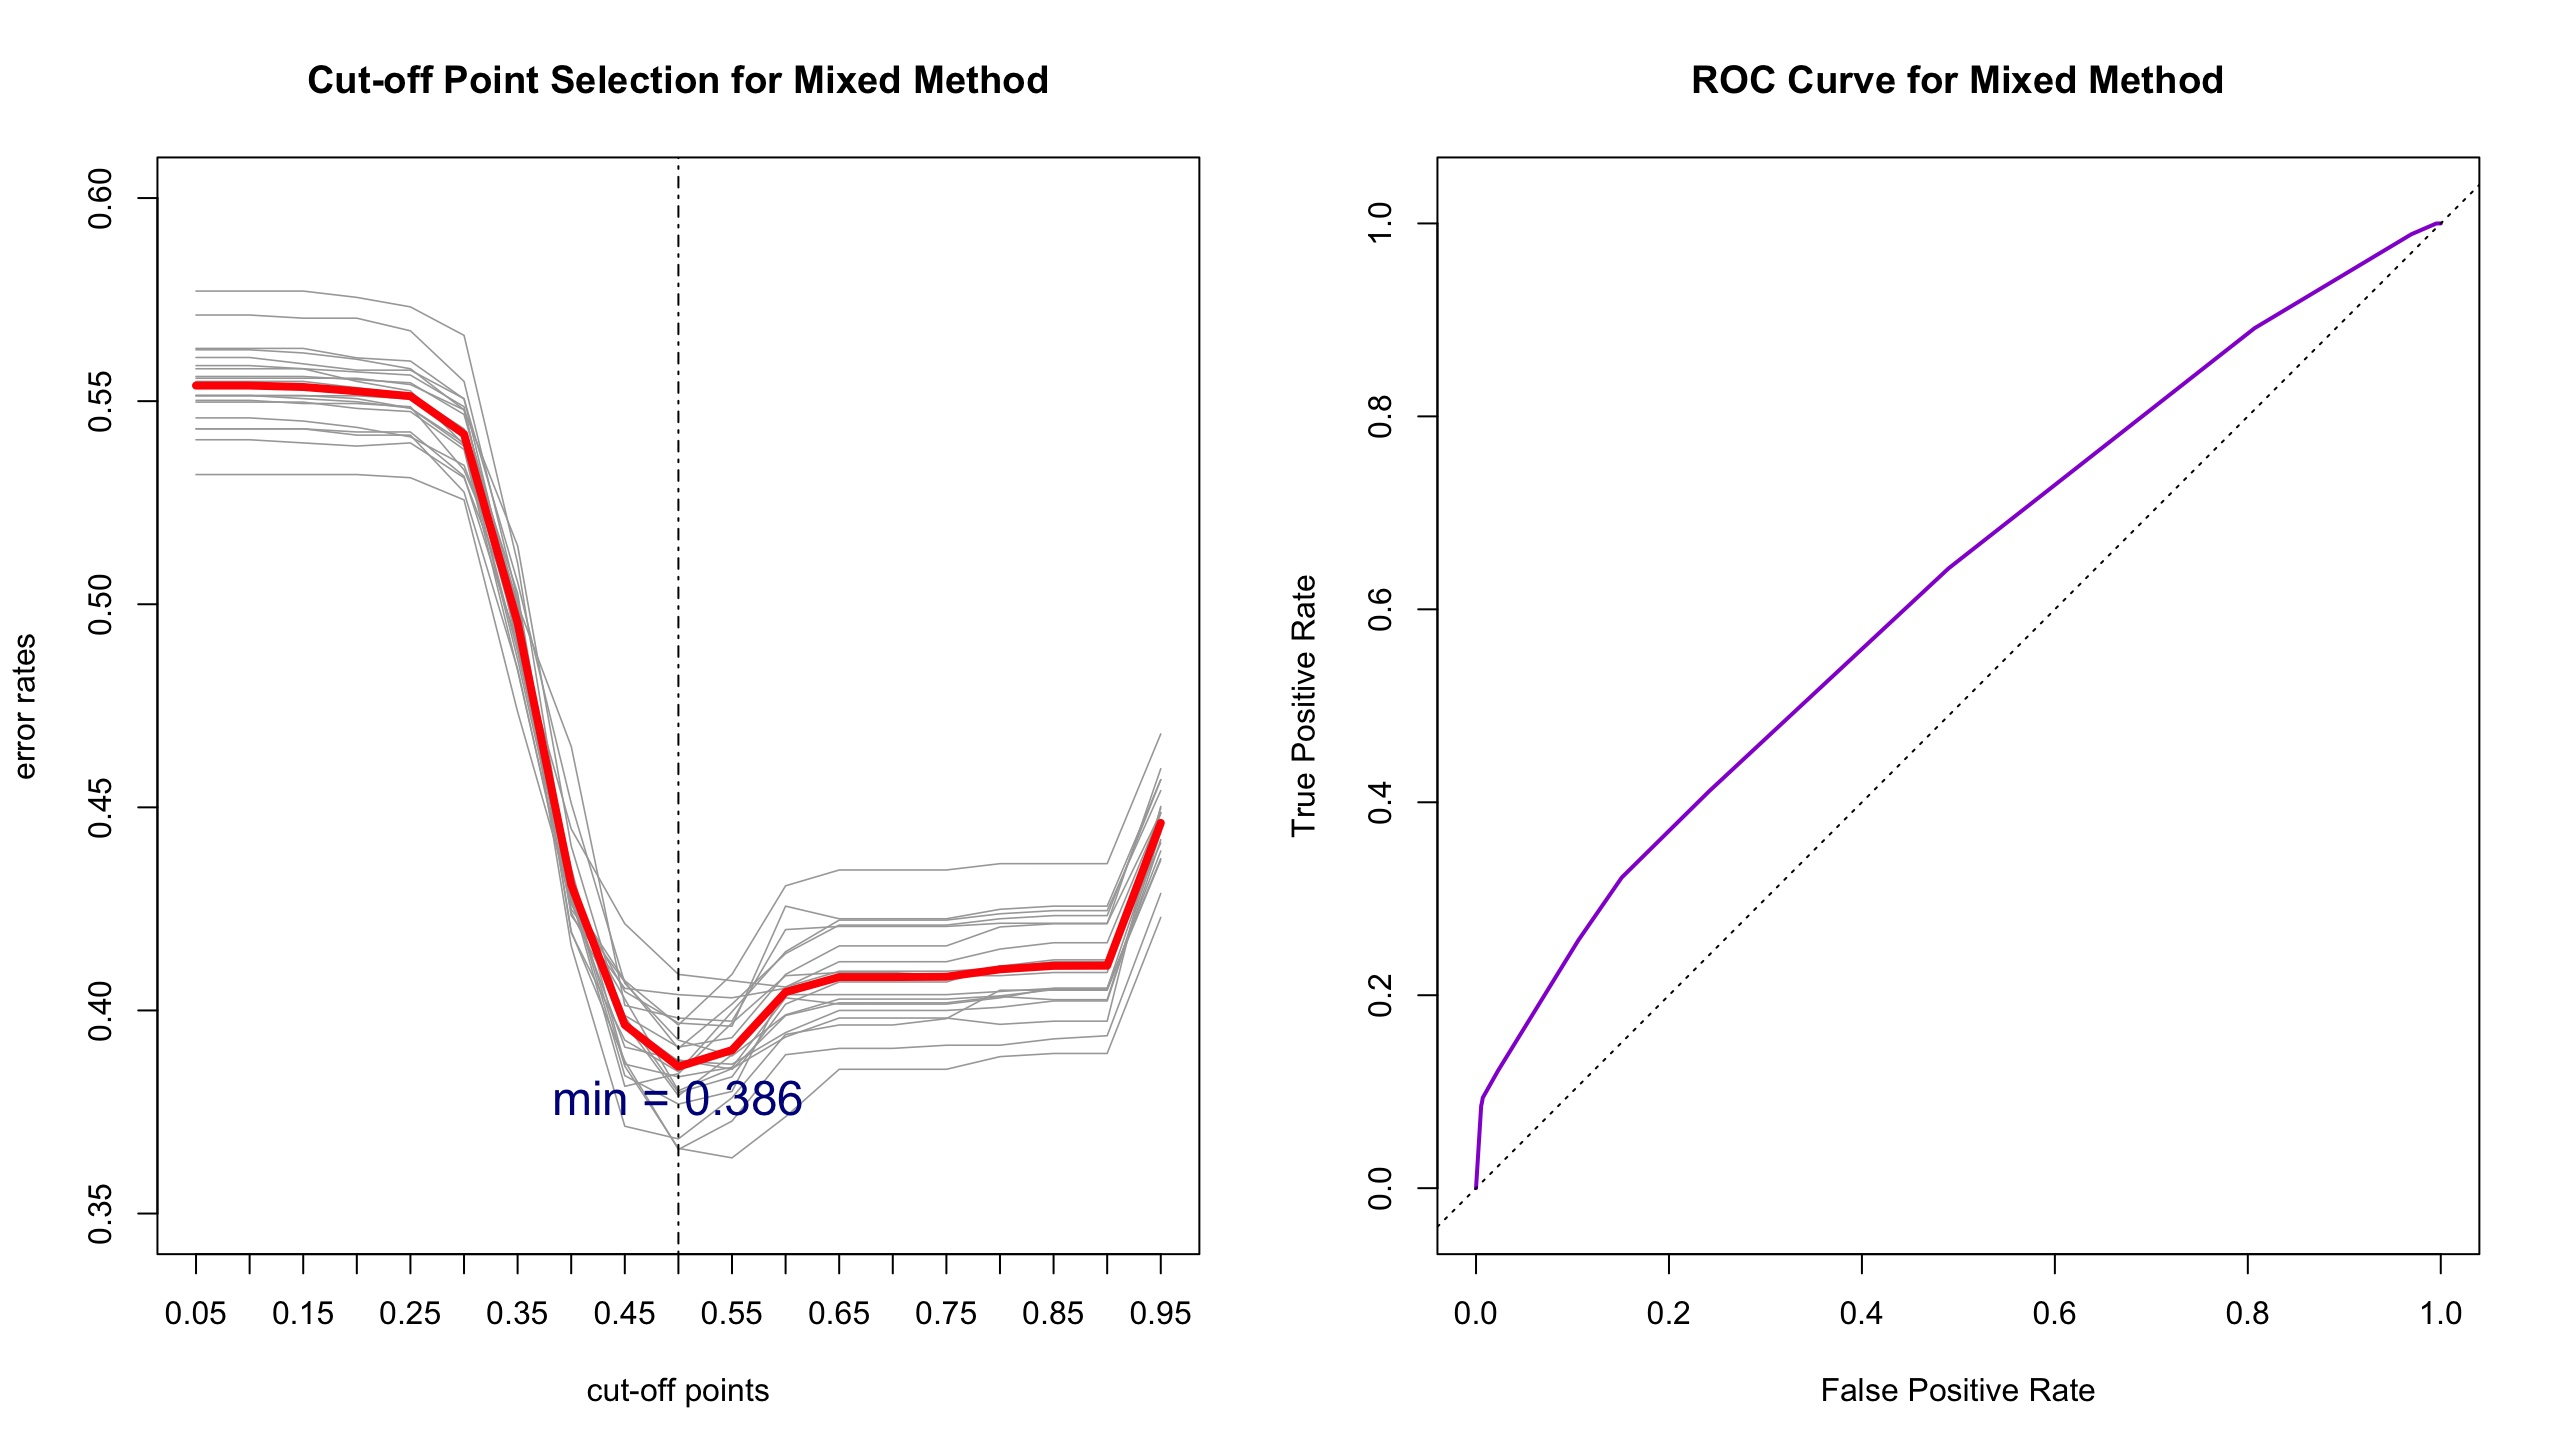
\includegraphics[width=300pt]{figure/f11_mixed_err.png}
    		\end{center}
	\end{figure}
}

%% lasso %%
\subsection{Logistic Lasso Regression}
% lasso1
\frame{
\qquad Now we introduce another model selection method, LASSO (least absolute shrinkage and selection operator) regression. After performing cross validation, we have the best $\lambda = 0.000546$ which has the model provide the least test error rate.
	\begin{columns}
		\begin{column}{0.5\textwidth}
\begin{table}[htp]
		\begin{center}
			\begin{tabular}{cr}
				predictor			&	coefficient		\\ \hline
				Intercept 			&	 0.19113 		\\ 
				Dunk    			&	-1.69536     	\\ 
				Jump Shot 		&	-0.28377		\\ 
				Tip Shot     		&	-0.20894     	\\  
				Shot Distance		&	-0.02038		\\ 
				Time Remaining     	&	 0.00002     	\\ 
			\end{tabular}
		\end{center}
	\label{default}
\end{table}			
		\end{column}		
		\begin{column}{0.5\textwidth}
			\begin{figure}
 		   		\begin{center}
		        			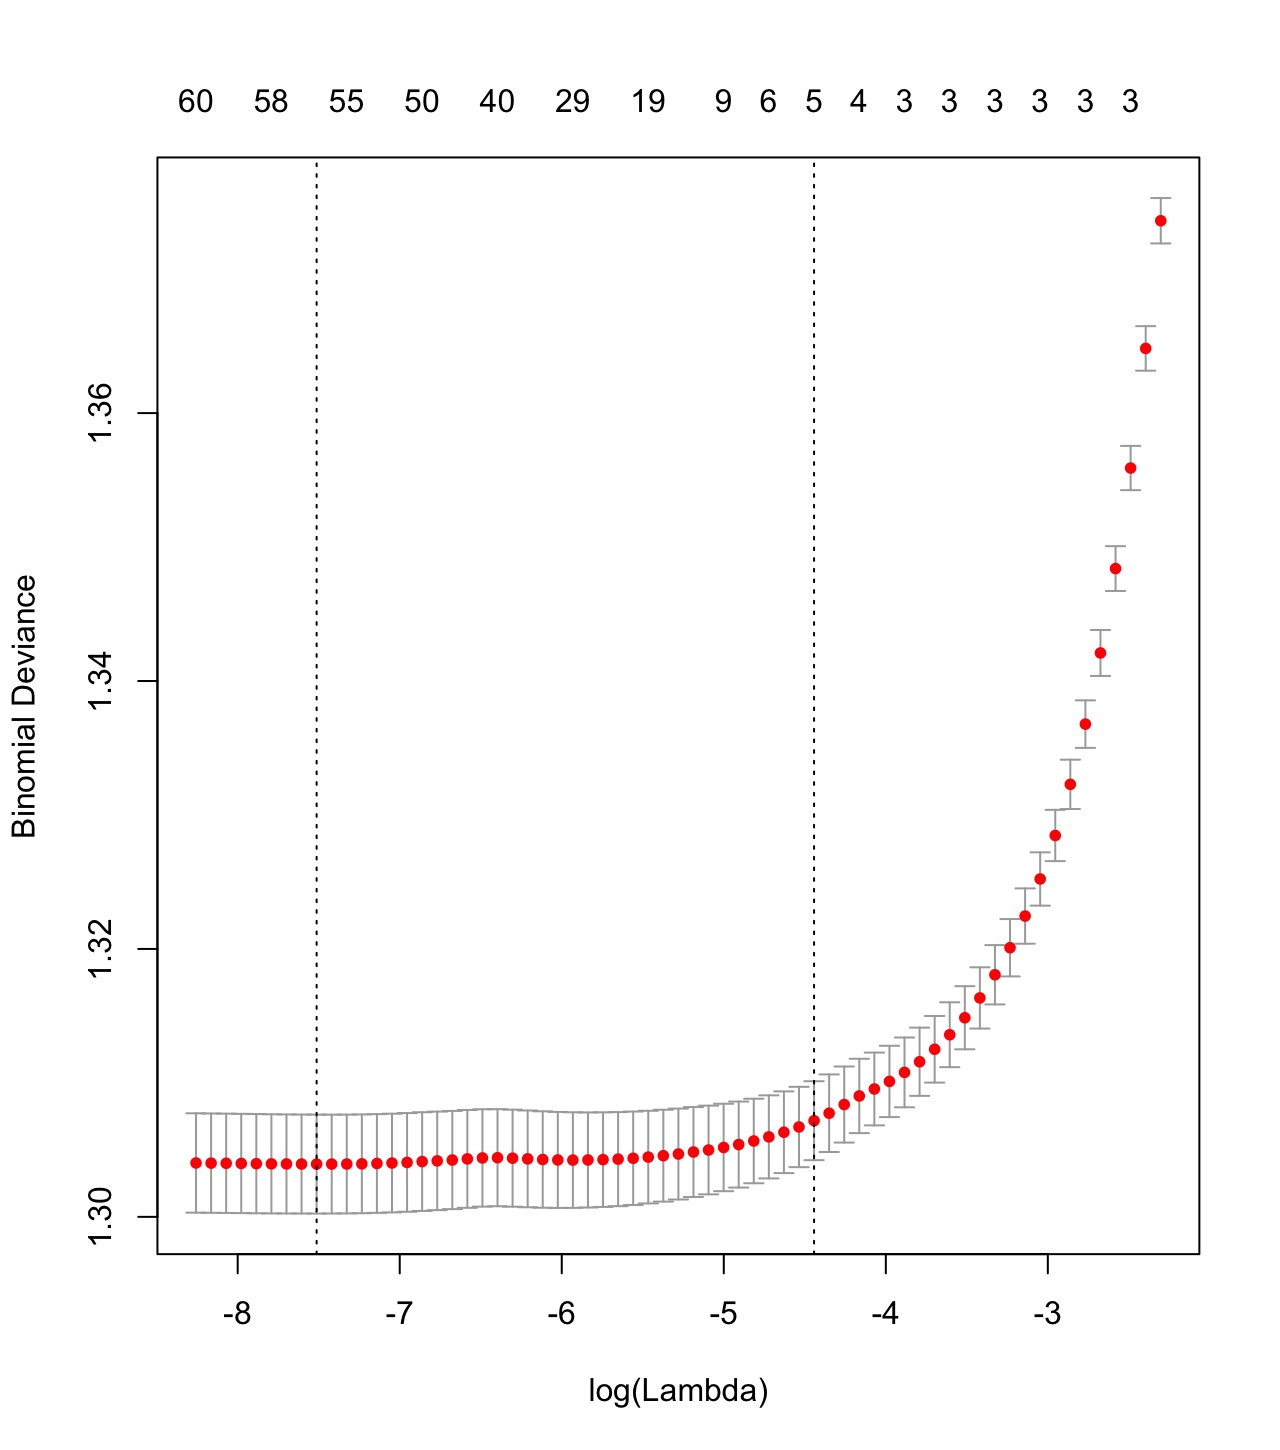
\includegraphics[width=123pt]{figure/f15_lasso_1.png}
   		 		\end{center}
			\end{figure}			
		\end{column}	
	\end{columns}

}
% lasso2
\frame{
	\begin{figure}
    		\begin{center}
        			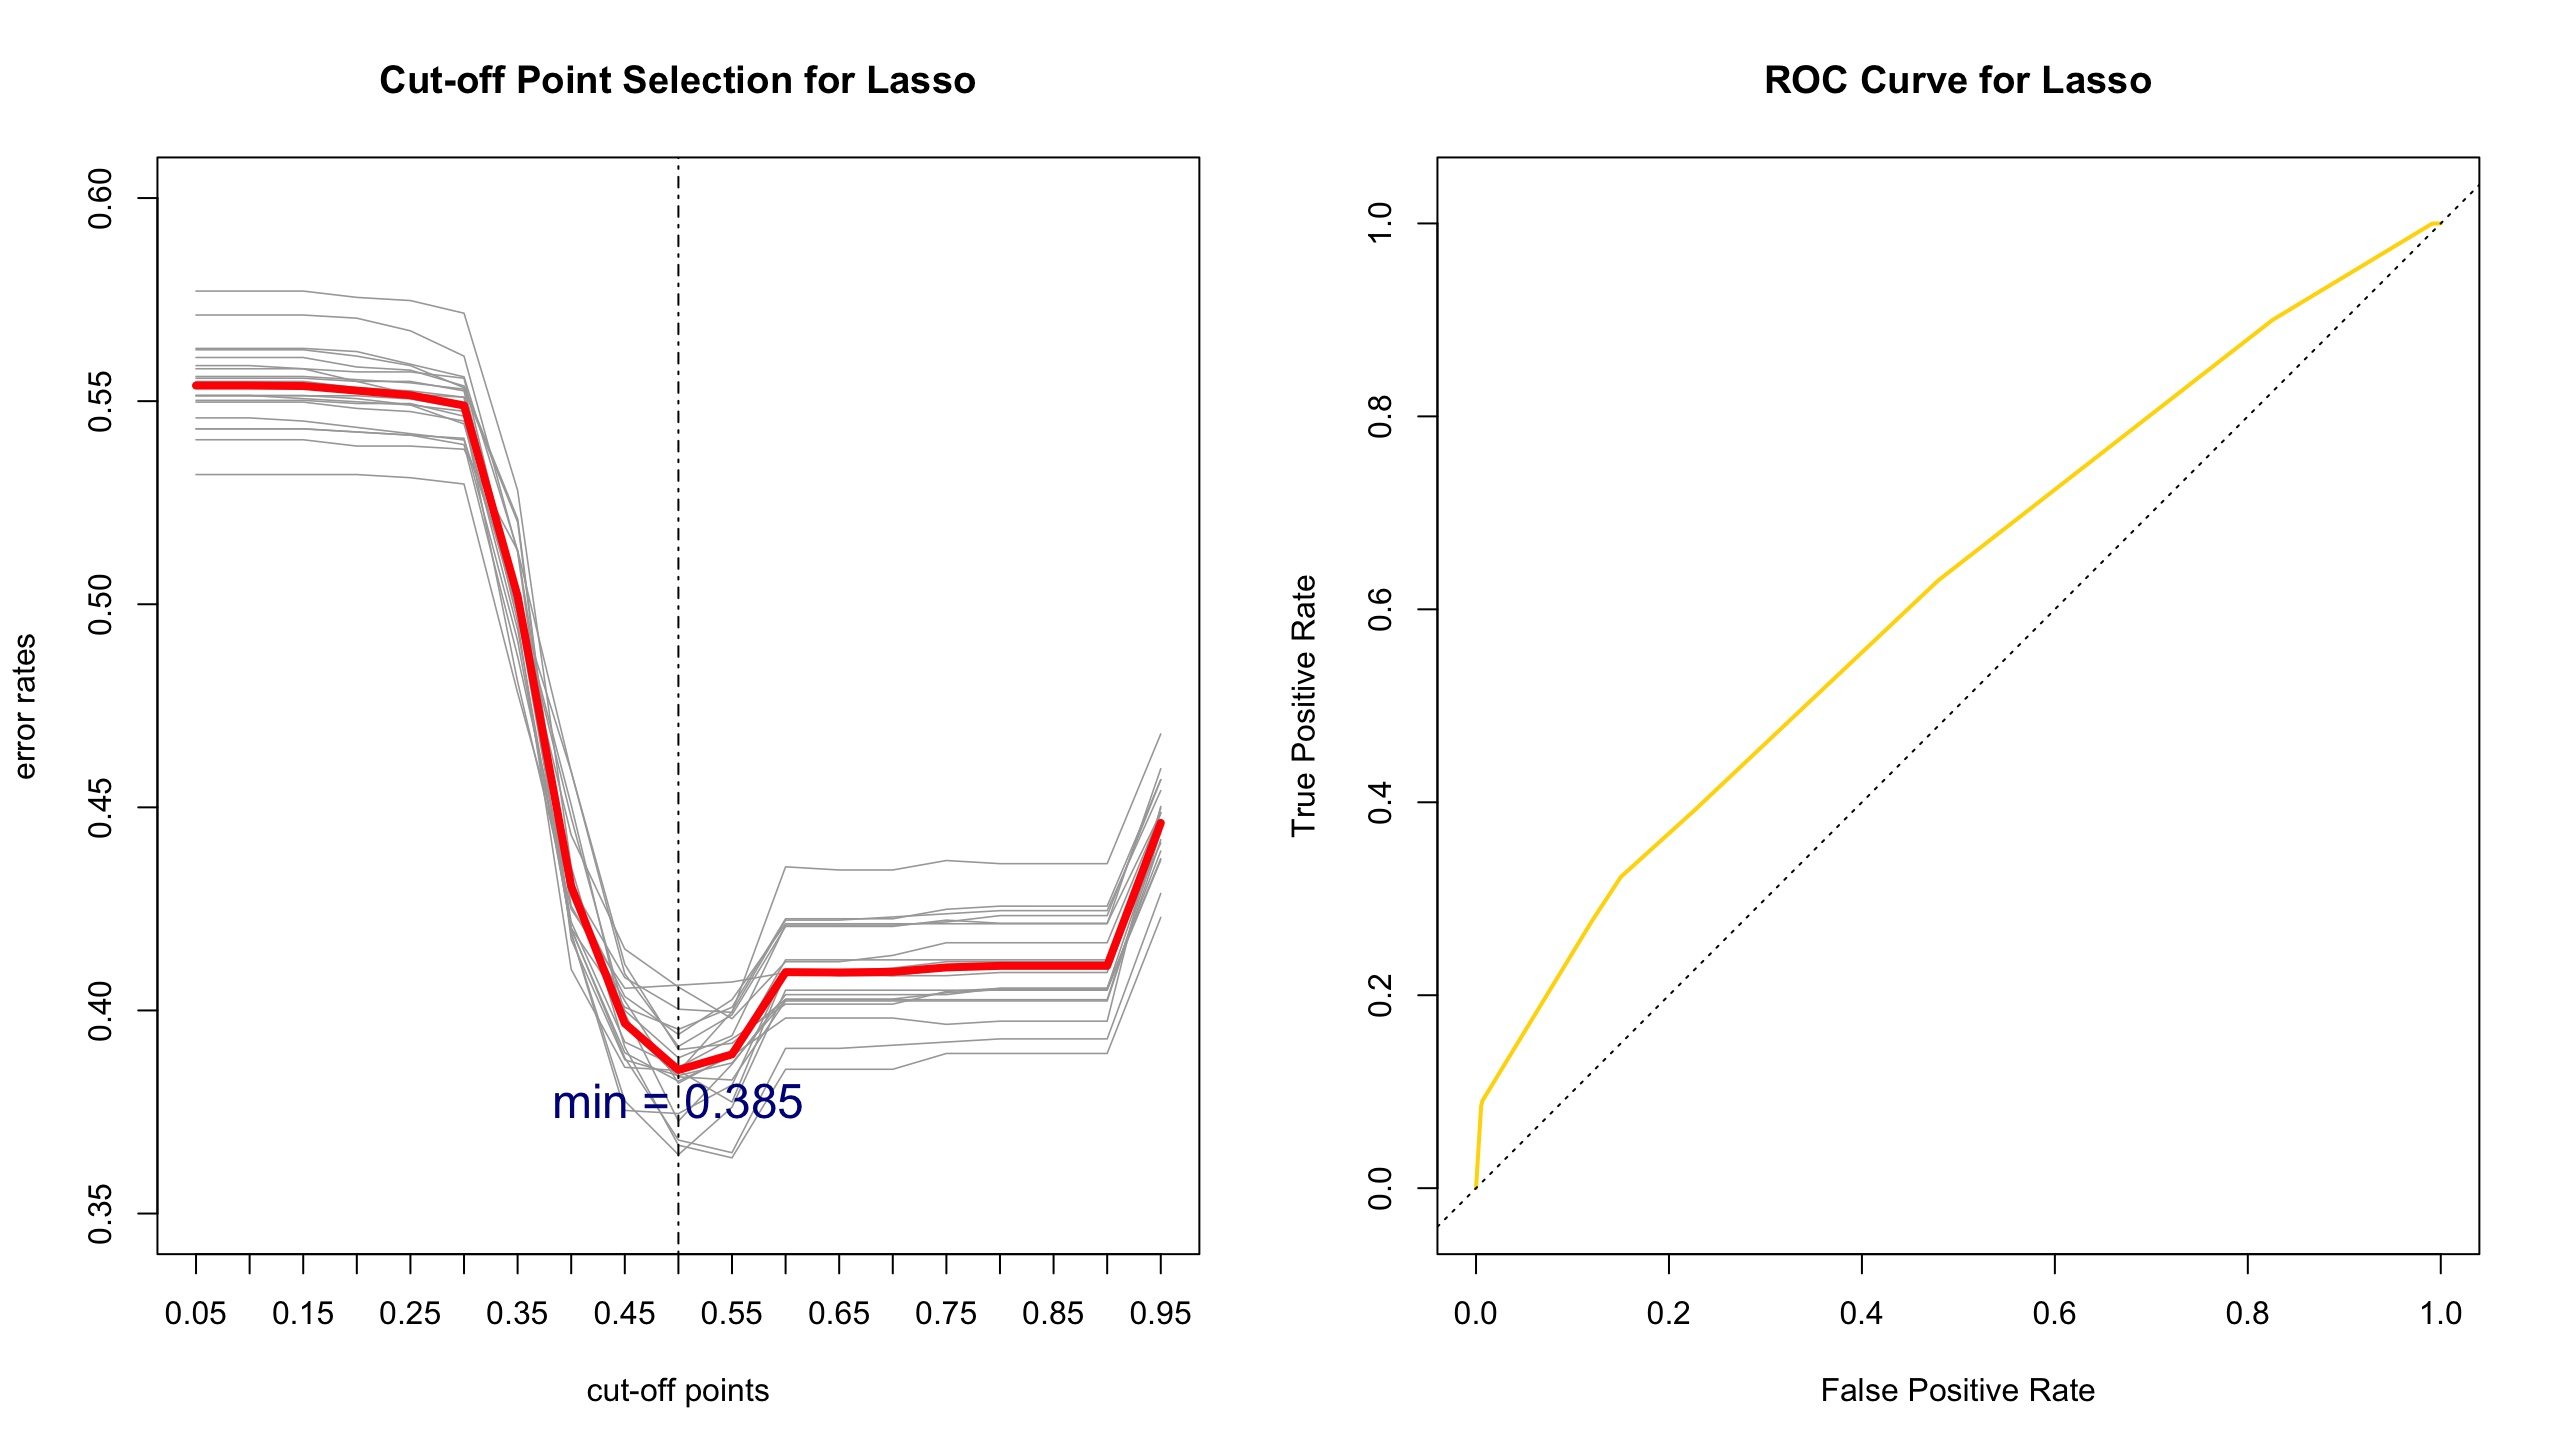
\includegraphics[width=300pt]{figure/f16_lasso_2.png}
    		\end{center}
	\end{figure}
}

%%%% Random Forest %%%%
\subsection{Random Forest}
\frame{
\qquad We applied random forest with 500 trees and derived 20-folds cross validation test error rate. The figure in the next slide shows that test error rates under the different $m$, the numbers of variables randomly sampled as candidates at each split. Notice that the Bagging(bootstrap and aggregating) method is a special case of the random forest with $m = 11$, the number of the predictors.
}

\frame{
	\begin{figure}
    		\begin{center}
        			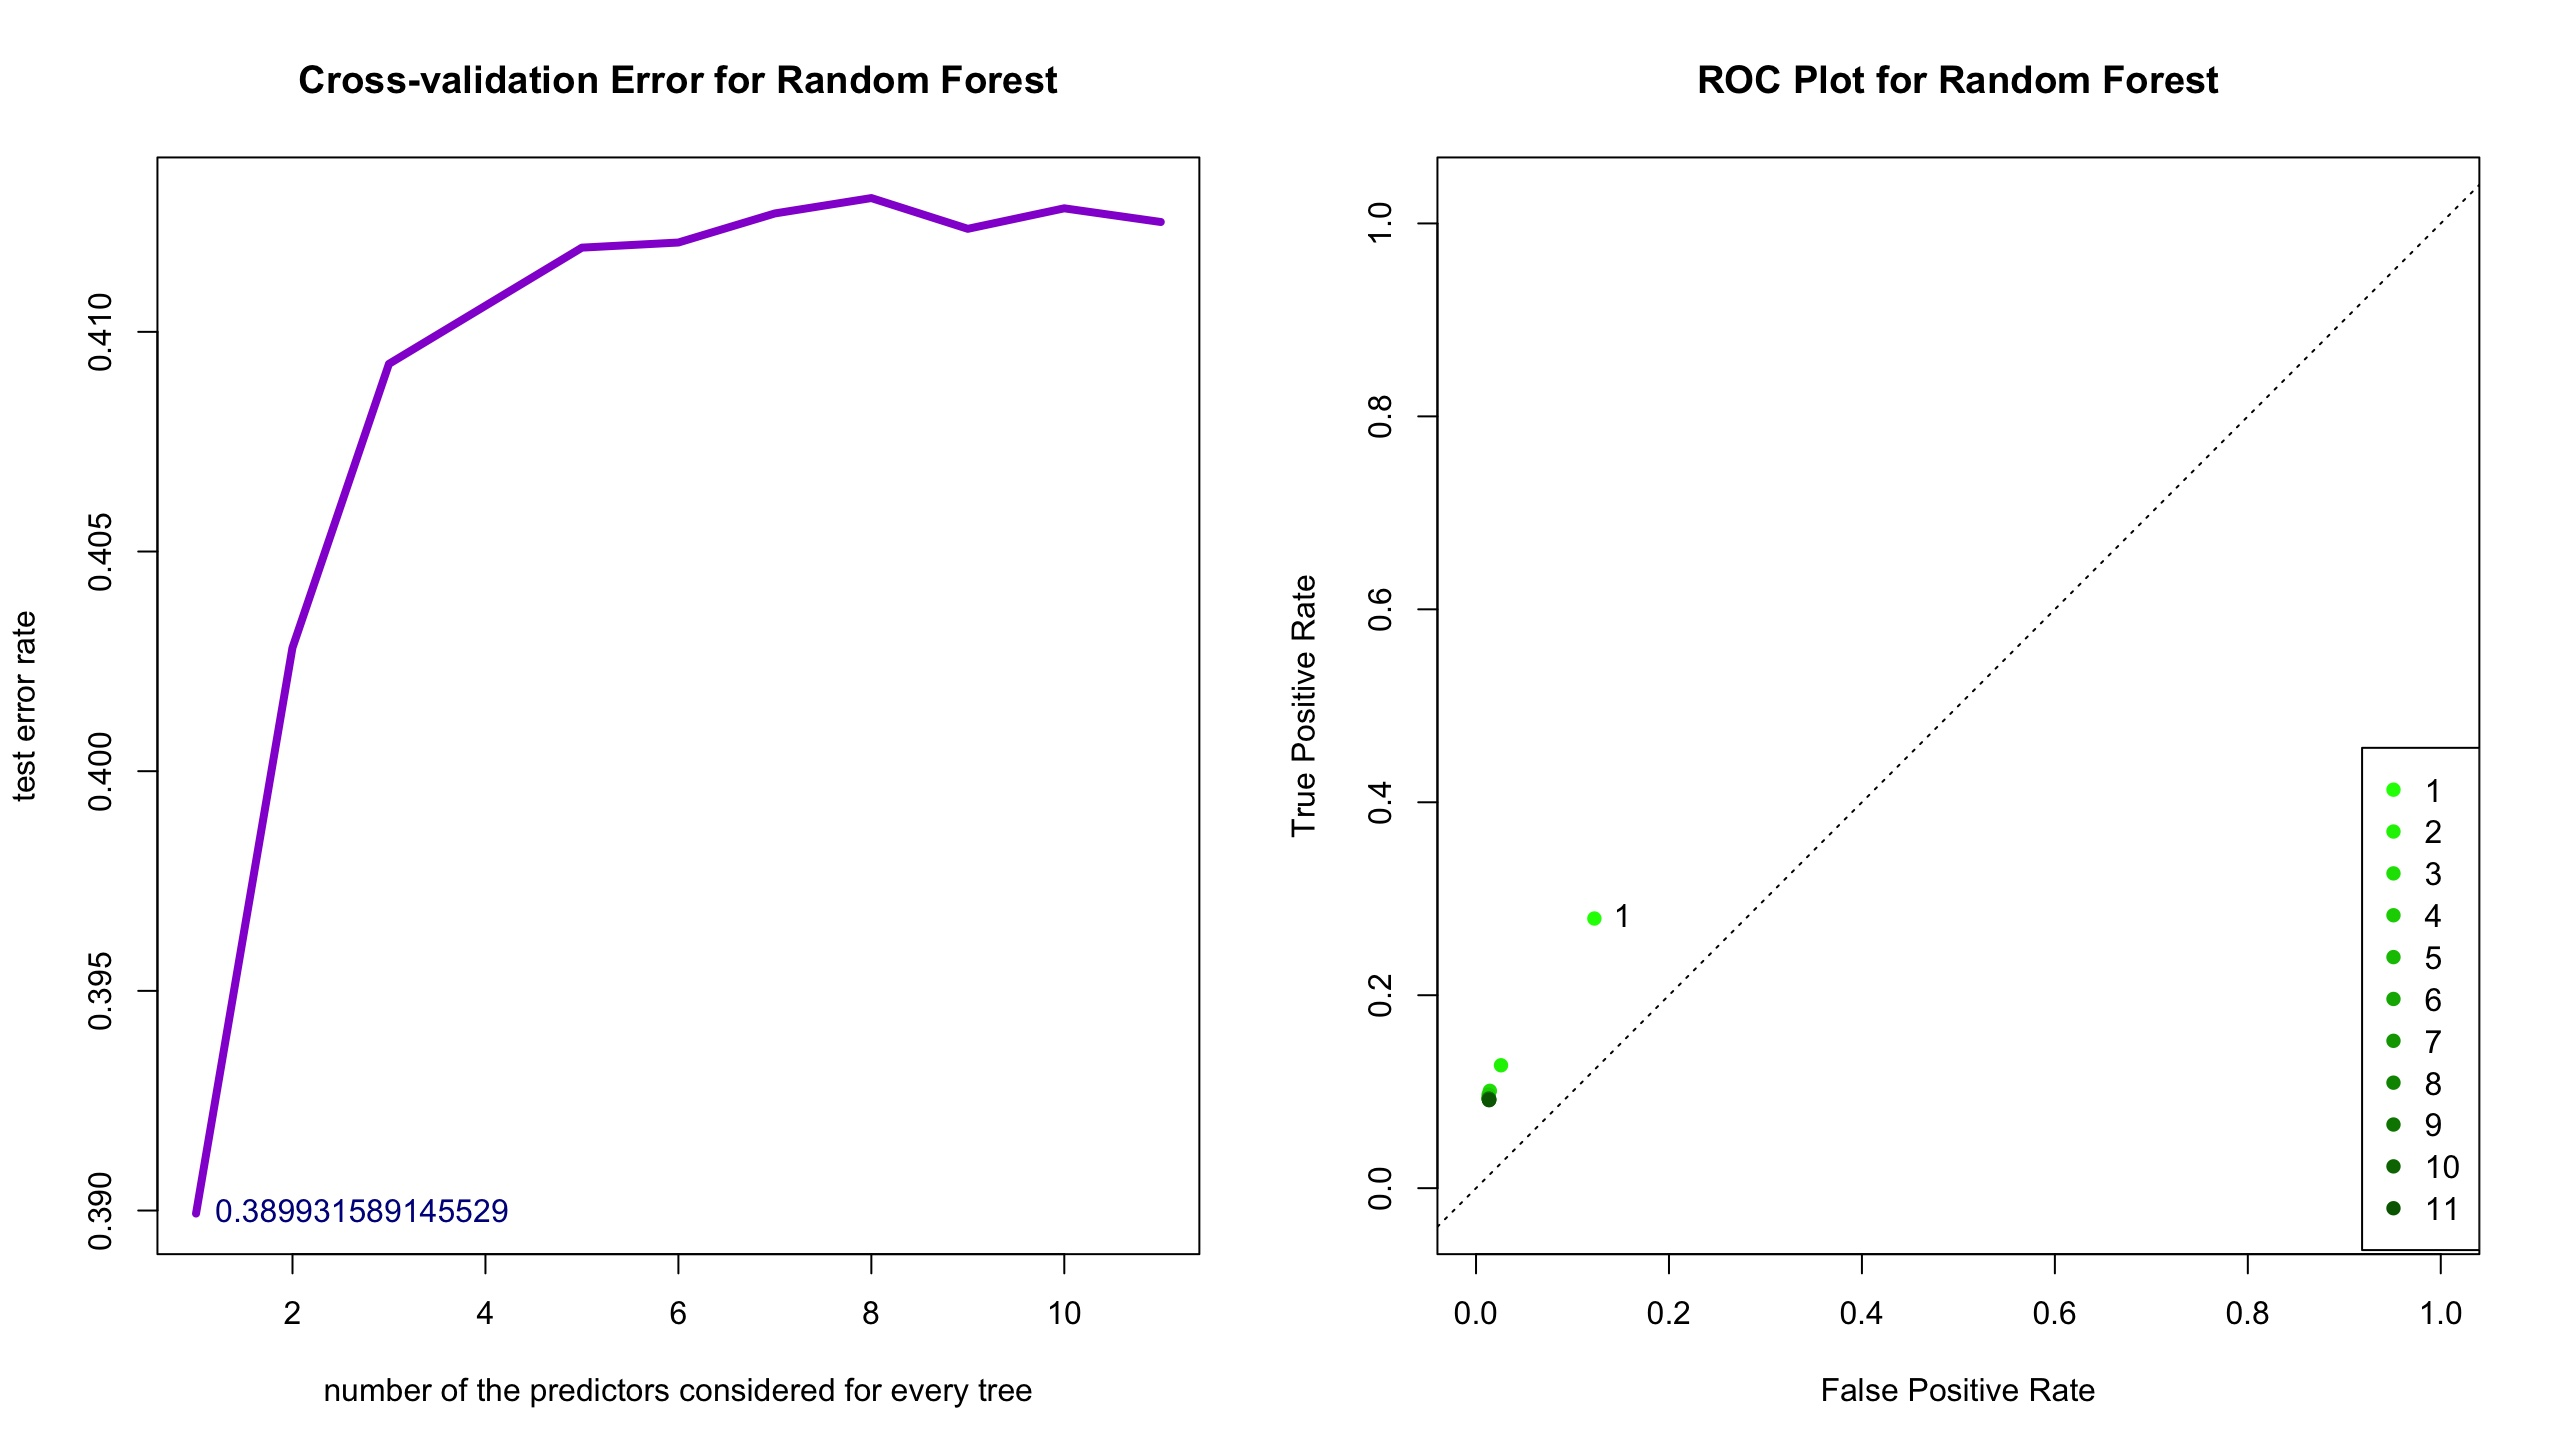
\includegraphics[width=300pt]{figure/f17_RF.png}
    		\end{center}
	\end{figure}
}

\frame{
\qquad The random forest with $m = 1$ performed the least test error rate among the 11 forests. Yet, the result is slightly worse than the one of the logistic regression.}

%%%% conclution %%%%
\section{Conclusion}
\subsection{Comparison of All Methods}
\frame{
	\begin{columns}
		\begin{column}{0.45\textwidth}
\qquad Comparing the ROC curves, we noticed that curves of all the methods excluding the KNN's coincide. Also 
the cross validation test error rates are about 0.385. Thus, we speculate that the models have reach their irreducible error.
	\end{column}		
		\begin{column}{0.55\textwidth}
			\begin{figure}
 		   		\begin{center}
		        			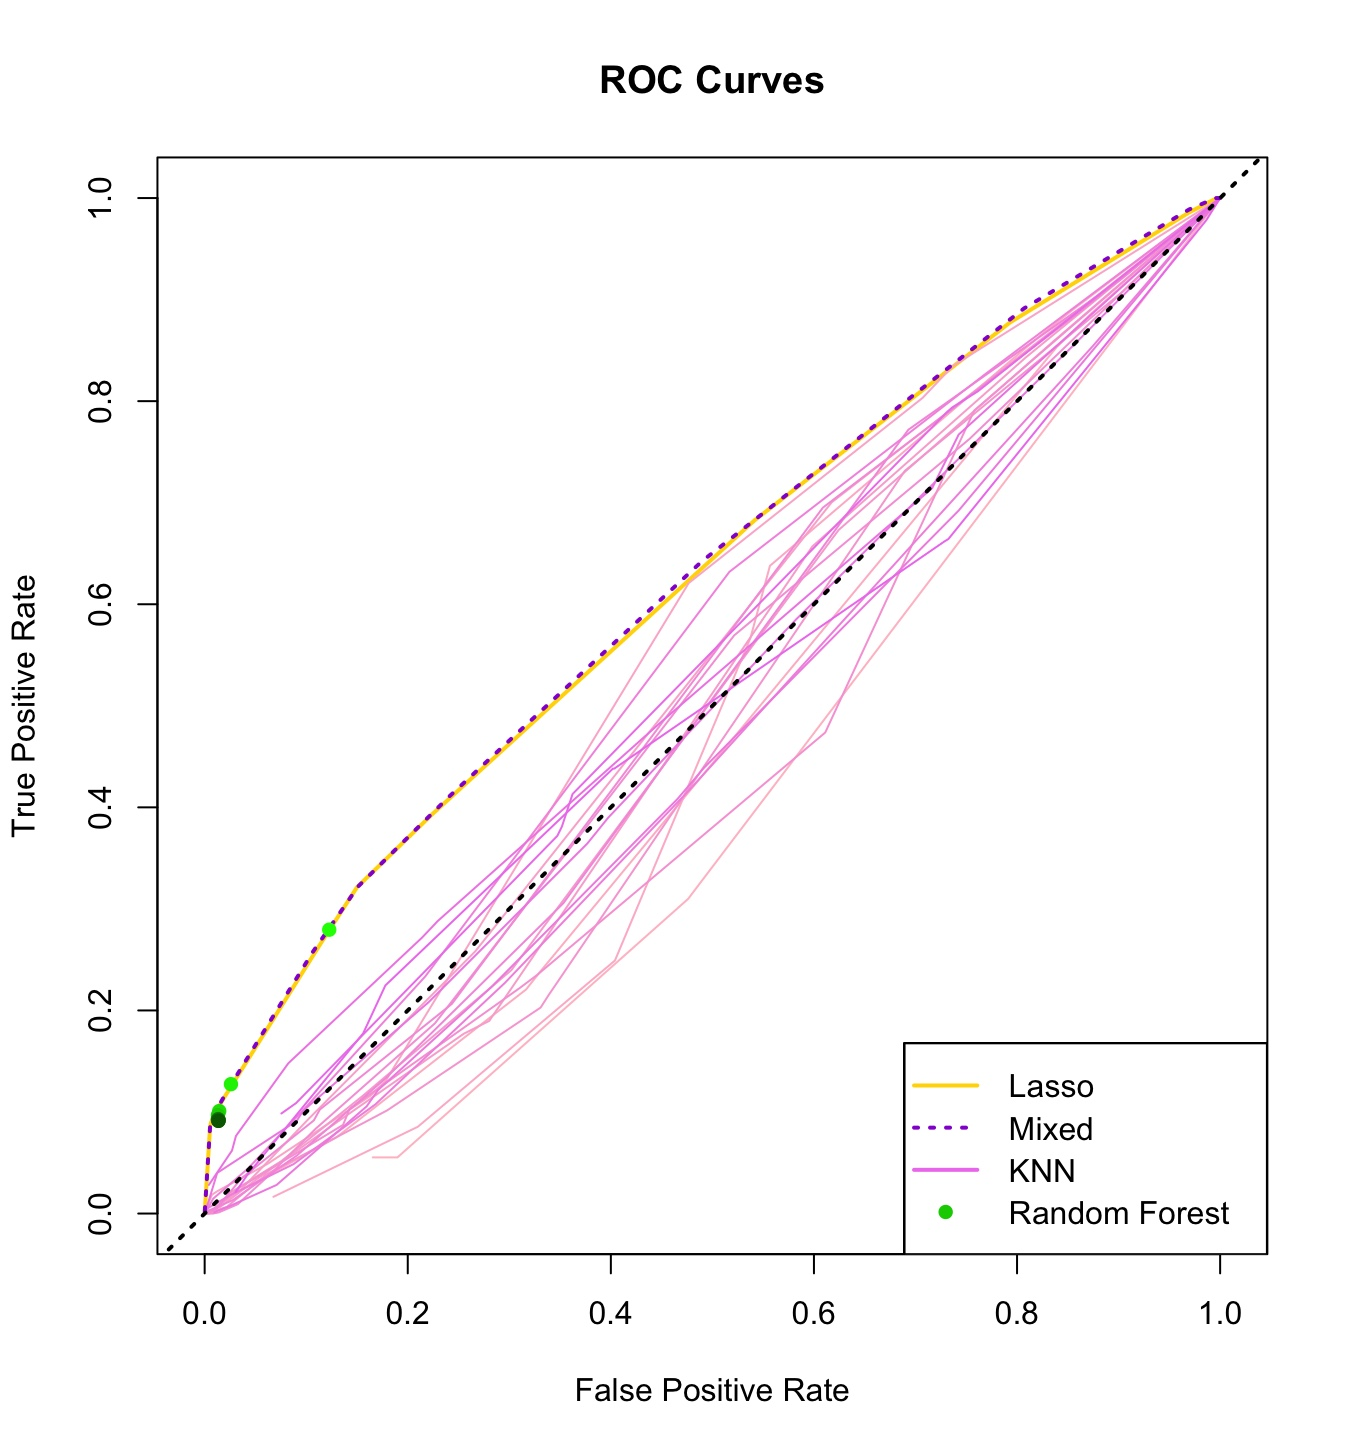
\includegraphics[width=180pt]{figure/f18_ROC.png}
   		 		\end{center}
			\end{figure}			
		\end{column}	
	\end{columns}
}

\subsection{Future Work}
\frame{
\begin{itemize}
	\item{Consider the support vector machine}
	\item{Collect data with more variable}
	\item{Give up}
\end{itemize}
}

\section{Reference}
\frame{
\begin{itemize}
	\item[1]{James, G., Witten, D., Hastie, T., Tibshirani, R., \textit{An Introduction to Statistical Learning with Applications in R}, Springer, New York, 2013}
	\item[2]{Kaggle, \textit{Kobe Bryant Shot Selection}, https://www.kaggle.com/c/kobe-bryant-shot-selection}
\end{itemize}	
}
\end{document}
